%%% LaTeX Template: Two column article
%%%
%%% Source: http://www.howtotex.com/
%%% Feel free to distribute this template, but please keep to referal to http://www.howtotex.com/ here.
%%% Date: February 2011

%%% Preamble
\documentclass[DIV=calc,%
              paper=a4,%
              fontsize=11pt,%
              onecolumn]{scrartcl}              % KOMA-article class

\usepackage{lipsum}                          % Package to create dummy text

\usepackage[italian]{babel}                    % Italian language/hyphenation
\usepackage[utf8]{inputenc}
\usepackage[protrusion=true,expansion=true]{microtype}        % Better typography
\usepackage{amsmath,amsfonts,amsthm}          % Math packages
\usepackage[pdftex]{graphicx}                  % Enable pdflatex
\usepackage[svgnames]{xcolor}                  % Enabling colors by their 'svgnames'
\usepackage[hang, small,labelfont=bf,up,textfont=it,up]{caption}  % Custom captions under/above floats
\usepackage{epstopdf}                        % Converts .eps to .pdf
\usepackage{subfig}                          % Subfigures
\usepackage{booktabs}                        % Nicer tables
\usepackage{fix-cm}                          % Custom fontsizes



%%% Custom sectioning (sectsty package)
\usepackage{sectsty}                          % Custom sectioning (see below)
\allsectionsfont{%                              % Change font of al section commands
  \usefont{OT1}{phv}{b}{n}%                    % bch-b-n: CharterBT-Bold font
  }

\sectionfont{%                                % Change font of \section command
  \usefont{OT1}{phv}{b}{n}%                    % bch-b-n: CharterBT-Bold font
  }



%%% Headers and footers
\usepackage{fancyhdr}                        % Needed to define custom headers/footers
  \pagestyle{fancy}                            % Enabling the custom headers/footers
\usepackage{lastpage}

% Header (empty)
\lhead{}
\chead{}
\rhead{}
% Footer (you may change this to your own needs)
\lfoot{\footnotesize \texttt{Progetto di Sistemi Intelligenti} \textbullet ~A.A. 2011/2012}
\cfoot{}
\rfoot{\footnotesize pagina \thepage\ di \pageref{LastPage}}
\renewcommand{\headrulewidth}{0.0pt}
\renewcommand{\footrulewidth}{0.4pt}



%%% Creating an initial of the very first character of the content
\usepackage{lettrine}
\newcommand{\initial}[1]{%
     \lettrine[lines=3,lhang=0.3,nindent=0em]{
            \color{DarkGoldenrod}
            {\textsf{#1}}}{}}



%%% Title, author and date metadata
\usepackage{titling}                              % For custom titles

\newcommand{\HorRule}{\color{DarkGoldenrod}%      % Creating a horizontal rule
                      \rule{\linewidth}{1pt}%
                    }

\pretitle{\vspace{-30pt} \begin{flushleft} \HorRule
        \fontsize{50}{50} \usefont{OT1}{phv}{b}{n} \color{DarkRed} \selectfont
        }
\title{Progetto di \\ Sistemi Intelligenti}          % Title of your article goes here
\posttitle{\par\end{flushleft}\vskip 0.5em}

\preauthor{\begin{flushleft}
          \large \lineskip 0.5em \usefont{OT1}{phv}{b}{sl} \color{DarkRed}}
\author{F. Disperati, D. Pellegrino, N. Redini, }                      % Author name goes here
\postauthor{\footnotesize \usefont{OT1}{phv}{m}{sl} \color{Black}
          University of Pisa                   % Institution of author
          \vskip 1em
          Anno Accademico 2011/2012
          \par\end{flushleft}\HorRule}

\date{}                                        % No date

\begin{document}

\maketitle
\clearpage

\tableofcontents
\clearpage

\section{Introduzione}
\subsection{Analisi del problema}
% The first character should be within \initial{}
\initial{I}l progetto consiste nell'applicazione delle tecniche di Computational Intelligence alla predizione dei consumi energetici di un edificio, adibito ad uffici, relativamente all'impianto di illuminazione.

Lo scopo è quello di predire l'andamento dei consumi e della luminosità all'interno di un edificio implementando quattro diverse tecniche di computational intelligence.

I dati raccolti sono stati sistemati in forma tabellare e riguardano i consumi registrati in 30 giorni tra maggio/giugno 2005. In particolare un singolo campione è costituito da:

\begin{itemize}
  \item Giorno
  \item Mese
  \item Anno
  \item Ora
  \item Minuto
  \item Irraggiamento solare esterno dall'edificio
  \item Luminosità rilevata nell'ambiente monitorato
  \item Energia media consumata
  \item Tipo di giorno (lavorativo/festivo)
\end{itemize}

La luminosità interna viene misurata in $Lux$ ed è stata monitorata attraverso un sensore, l’irraggiamento solare viene rappresentato in $W/m^2$ ed indica la quantità di radiazione solare per unità di superficie; infine l'energia consumata è espressa in $W/h$.


\subsection{Analisi dei dati}
Dal momento che le tecniche che andremo ad analizzare richiedono delle particolari strutture in ingresso, il primo passo è dunque lo studio dei dati forniti atto all'ottimizzazione della struttura interna del modello.

Per prima cosa è doveroso far presente che nei dati è presente un errore nel sample inerente al 30 maggio ( un lunedì ); infatti come è possibile vedere dai dati, tale giorno è marcato come festivo.

Si è dapprima supposto che si trattasse di una qualche festività ( ad esempio il 30 maggio ricorreva il Memorial Day negli U.S.A. ), ma osservando i dati di consumo rilevati, si è subito capito che si trattava semplicemente di un errore.

Un primo possibile approccio risolutivo poteva essere quello di correggere a mano l'errore, bensì vedremo a breve come è stato affrontato il problema.

Osservando i dati si nota che l'anno in questione non cambia ( sono stati campionati solo due mesi ), è dunqe plausibile pensare che l'ingresso 'Anno' non influenzi l'output delle reti che andremo a modellare, e che quindi sia del tutto superfluo; motivo per cui è stato rimosso.

Inoltre, per migliorare le performances delle reti modellate, i dati sono stati mediati con steps di un ora, elimimando quindi anche l'ingresso Minuti; in questo modo gli effetti sulla rete di eventuali picchi anomali (tra i dati campionati) vengono attenuati.

Infine si è scelto di suddividere i due mesi in settimane ( da 1 a 8 ) ed i giorni in “giorni setttimanali” ( da 1 a 7 ); così facendo è stato possibile eliminare l'ingresso 'Tipo di giorno'.

Quest'ultima operazione è stata possibile secondo la seguente considerazione: se il giorno è festivo (sabato o domenica) i consumi energetici sono pressochè nulli, cosa che non accade quando il giorno è lavorativo ( da lunedi a venerdi). 

In sostanza abbiamo trasportato l'informazione che forniva l'ingresso 'Tipo di giorno' al numero di giorno della settimana; sarà poi compito della rete apprendere l'andamento dei consumi durante la settimana; così facendo è stato inoltre possibile correggere l'errore presente nei dati senza intervenire a mano.

Infine è importante notare che l'ingresso 'Tipo di giorno' non sarebbe divenuto inutile qualora nei mesi campionati fossero state presenti festività particolari ( Natale, Pasqua etc ).

Quanto fin'ora descritto è stato reso possibile attraverso lo script ruby sotto riportato.

\inputminted[linenos=true,fontsize=\footnotesize]{ruby}{../../data/conform.rb}
\captionof{listing}{data/conform.rb}


\clearpage


\section{Modelli di fitting}
\subsection{Rete neurale statica}
Il primo strumento che abbiamo utilizzato per lo studio del nostro modello si basa sulle reti di apprendimento di tipo neurale statiche, ovvero il tool Neural fitting di matlab.

Tale tool mette a disposizione dell'utente una semplice GUI la quale permette, attraverso pochi semplici passi di setup, la crezione di una rete neurale statica.

Nonostante tale procedimento sia estramemente semplice, i risultati desiderati possono essere ricavati dopo molte prove dovute a successivi allenamenti della rete ( fase di addestramento ) e a cambiamenti nella struttura interna quali ad esempio il numero di neuroni nascosti.

In particolare la fase di addestramento di una rete neurale prevede che la rete prenda in ingresso un vettore di inputs e ristituisca un risultato, il quale sarà confrontato quindi con un vettore “obiettivo” per verificarne la bontà dei valori ottenuti.

In base all’esito del confronto questa elaborazione viene ripetuta, modificando opportunamente i pesi su ciascun neurone, fino ad ottenere un livello di apprendimento accettabile.

Al fine di ottenere un apprendimento soddisfacente, ovvero che minimizzi l’errore dato dalla differenza tra il vettore obiettivo e il vettore dei risultati ed una retta di regressione il più possibile vicina all'unità, è stato deciso di creare uno script ed una funzione matlab per rendere la ricerca di una rete considerata “ottima” un processo automatico.

Prima di procedere con la spiegazione di tali scripts, è doveroso mostrare quale struttura è stata utilizzata per modellare la rete neurale.

Come possiamo vedere dalla figura sottostante essa prevede uno strato nascosto, composto in linea generale da un numero di neuroni impostabile dall'utente (12 nell'esempio), con funzione di attivazione sigmoide ed uno strato lineare di uscita.\\

\vspace{20px}
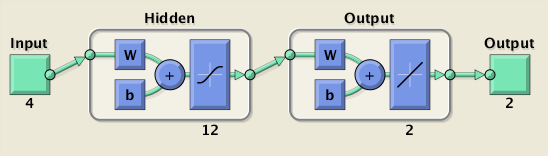
\includegraphics[scale=0.5]{images/neural_net/net.png}
\captionof{figure}[One figure]{Modello di rete neurale}
\vspace{20px}

\subsubsection{Ricerca della migliore rete neurale}
Nell'ottica di automatizzare il processo di modellizzazione della rete, è stata definita sia una funzione per la ricerca di una rete neurale statica considerata ottima, sia uno script per la visualizzazione dei risultati ottenuti.

\paragraph{Funzione searchBestFitting}
Essa provvede alla creazione di una rete neurale al suo addestramento, e all'estrazione dei parametri di interesse quali il coefficiente della retta di regressione ( nel caso test ) e le performances ( valutate sull'MSE ).

La funzione inizializza, e quindi allena, la rete neurale RETRAIN\_ATTEMPTS volte e restituisce alla fine la migliore rete trovata: ovvero quella che ha presentato nella fase di test i migliori parametri.

Chiaramente sono stati impostati anche due GOALs oltre cui la rete ricavata è considerata ottima, nello specifico si consiedera una rete ottima se i valori di regressione sono maggiori o uguale a 0.99 ed MSE minore di 1000.

Ad ogni passo i parametri discriminanti per la bontà della rete sono quelli della fase di test in quanto indicanti la capacità della rete di generalizzare, e dunque di aver correttamente appreso.

E' importante notare che dopo ogni RETRAIN\_ATTEMPTS la struttura interna della rete viene modificata variando il numero di neuroni dello strato nascosto, in modo da confrontare tra loro diverse configurazioni; infine la funzione di addestramento utilizzata è quella standard di backpropagation di Levenberg-Marquardt (trainlm).

La funzione appena esposta è la seguente:

\inputminted[linenos=true,fontsize=\footnotesize]{matlab}{../../src/neural\ network/functions/searchBestFitting.m}
\captionof{listing}{src/neural network/functions/searchBestFitting.m}


\paragraph{Script netfit}
Tale script si occupa semplicemente di inizalizzare il vettori inputs/outputs, richiamare la funzione appena illustrata e quindi stampare a schermo i risultati ottenuti.

In questo script viene inoltre fatto uso della funzione {\bf unix} di matlab per eseguire lo sript conform.rb per la creazione dei dati necessari alla funzione searchBestFitting.

\inputminted[linenos=true,fontsize=\footnotesize]{matlab}{../../src/netfit.m}
\captionof{listing}{src/netfit.m}


\subsubsection{Risultati}
I risultati ottenuti eseguendo lo script sono i seguenti:\\
\vspace{20px}

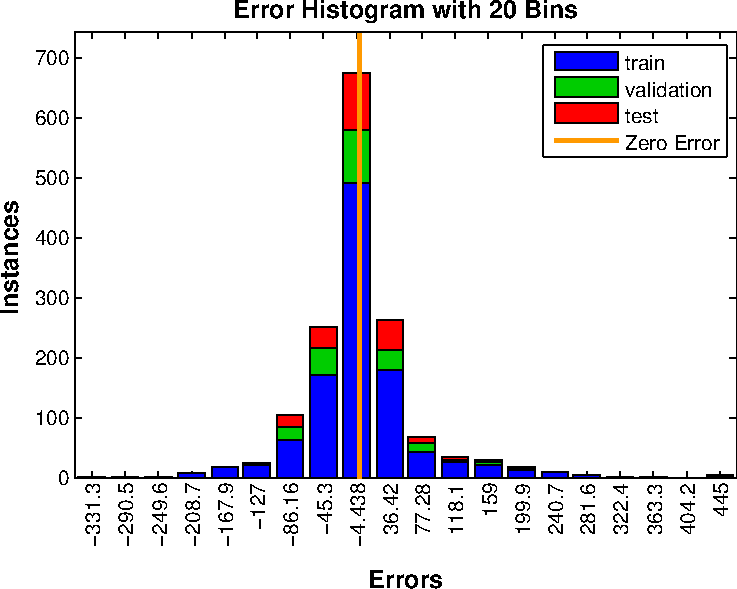
\includegraphics[scale=0.7]{images/neural_net/histogram.pdf}
\captionof{figure}[One figure]{Istogramma degli errori}
\vspace{20px}

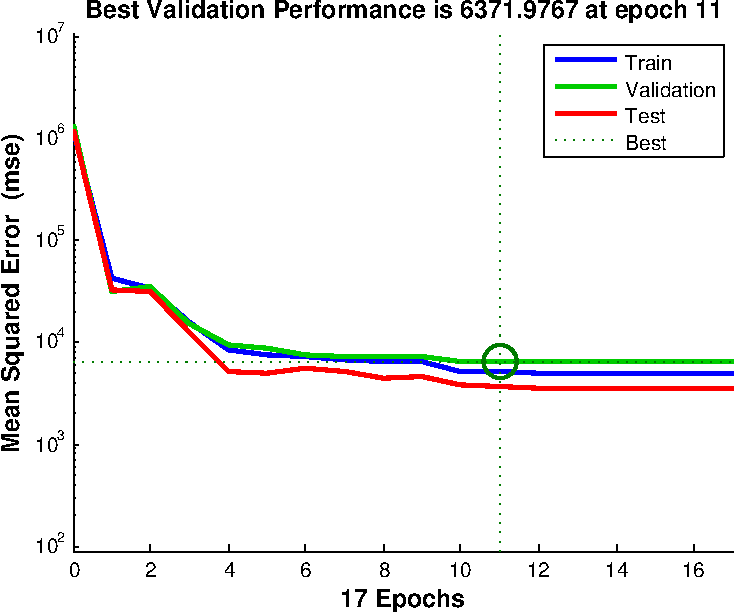
\includegraphics[scale=0.7]{images/neural_net/performances.pdf}
\captionof{figure}[One figure]{Prestazioni della rete (MSE)}
\vspace{20px}

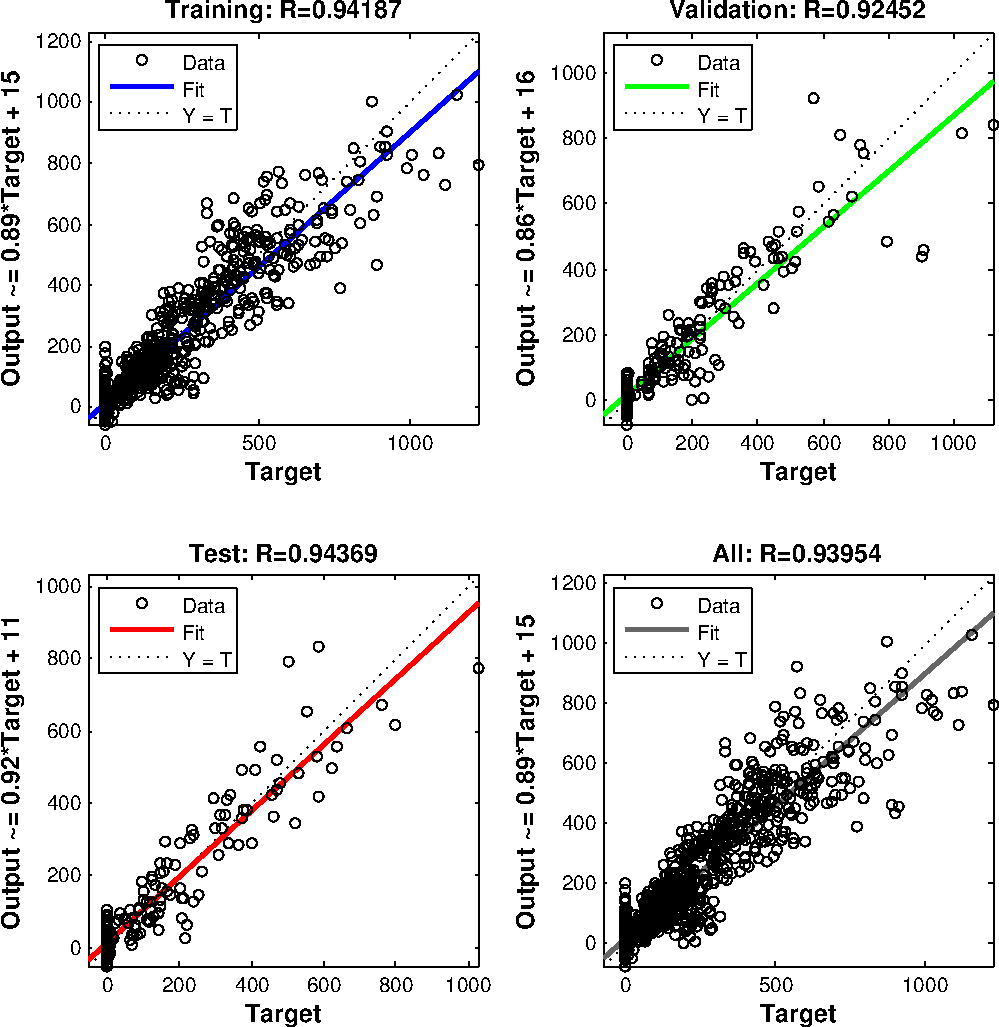
\includegraphics[scale=0.7]{images/neural_net/regressions.pdf}
\captionof{figure}[One figure]{Rette di regressione}
\vspace{20px}

\clearpage

\subsection{Fuzzy Network}

\subsubsection{Scelta del modello}
Il concetto base della logica fuzzy è quello di mappare uno spazio di ingresso in uno spazio di uscita sfruttando un elenco di relazioni if-then chiamate regole.

Tali regole si riferiscono a variabili e ad aggettivi che le descrivono. Prima di poter costruire un sistema che interpreti le regole, è necessario definire tutti i termini che si pensa di utilizzare e gli aggettivi che li descrivono.

Il Fuzzy Logic Toolbox (fuzzy) di Matlab permette di creare due tipi di Fuzzy Inference Systems (FIS) che si differenziano per il modo in cui le uscite sono determinate:

\begin{itemize}
  \item Mamdani
  \item Sugeno
\end{itemize}

Nel seguito faremo riferimento ad un FIS Mamdani-type completamente definito sfruttando la GUI proposta da Matlab dove si è scelto di mantenere le impostazioni di default per le principali funzioni logiche.

Una fase preliminare importante consiste nel valutare e selezionare, in base ai dati forniti, le variabili di input e di output.

Per quanto riguarda gli input, ad esempio, la suddivisione tra giorno festivo e giorno feriale non può essere rappresentata utilizzando un modello fuzzy in quanto la suddetta suddivisione è netta e solo la creazione di 2 modelli distinti permette di tenerne conto.

Per lo stesso motivo considereremo i vari giorni della settimana come equivalenti, eccezion fatta per i giorni festivi, escludendo così anche questa componente dagli ingressi.

In ingresso al sistema perciò avremo soltanto due variabili, l’ora del giorno e l’irraggiamento esterno, in quanto i dati forniti non giustificano l’utilizzo di nessun’altra variabile che andrebbe soltanto a complicare il modello.

Si definirà un FIS per ogni variabile di uscita del problema in modo tale da poter ottimizzare il modello su tale output; avremo quindi un totale di quattro sistemi, rispettivamente, per la predizione di:

\begin{itemize}
  \item Energia consumata nei giorni festivi;
  \item Energia consumata nei giorni feriali;
  \item Luminosità misurata nei giorni festivi;
  \item Luminosità misurata nei giorni feriali (nel seguito si farà riferimento a questo scenario nell'illustrazione del procedimento utilizzato per la realizzazione del modello Fuzzy).
\end{itemize}


\subsubsection{Definizione delle MFs}
In ingresso al sistema avremo perciò, come discusso precedentemente, soltanto due variabili, l'ora del giorno e l'irraggiamento.

Il modello avrà la seguente struttura:

\begin{figure}
  \centering
  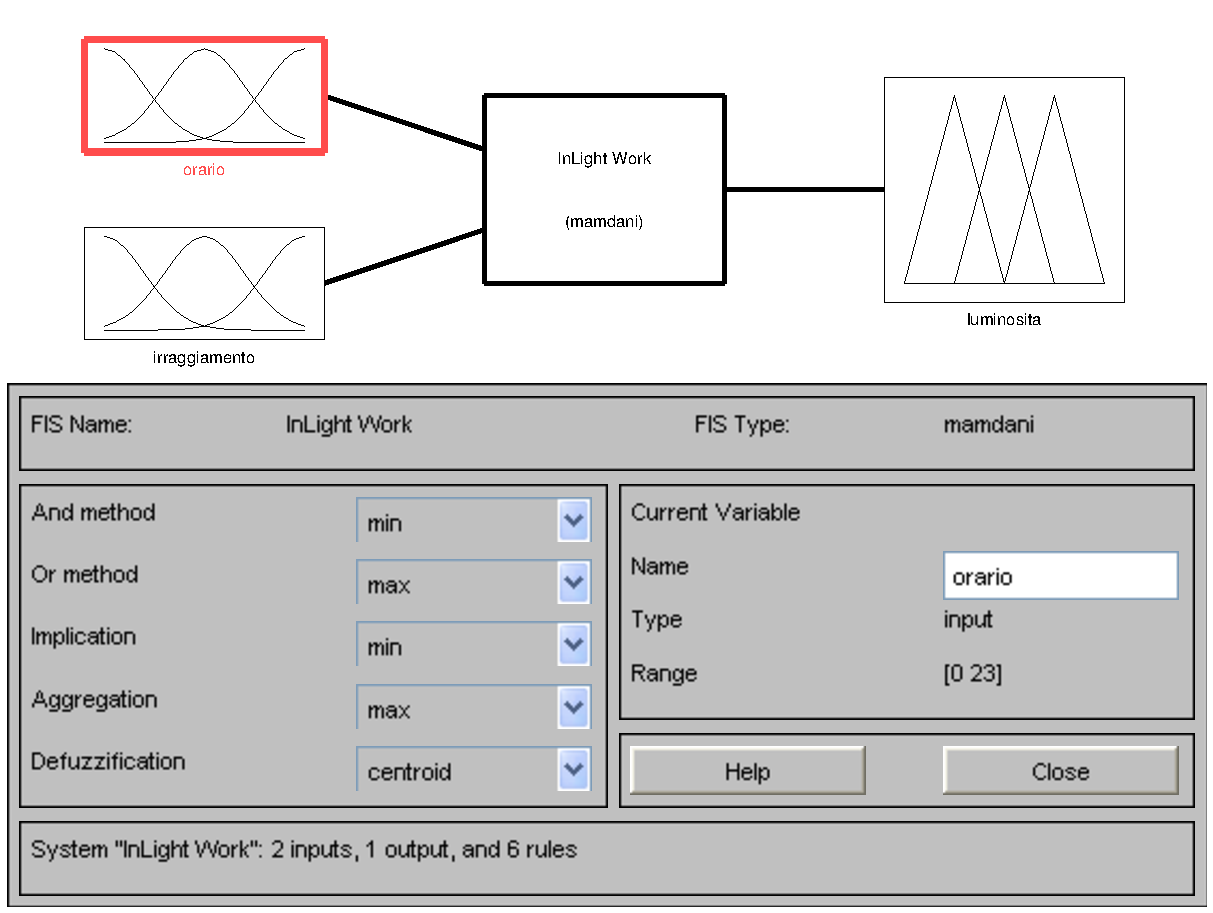
\includegraphics[scale=0.5]{images/fuzzy/modello_fuzzy_luminosita.pdf}
  \caption{Modello fuzzy luminosità}
\end{figure}

A questo punto è necessario analizzare ogni variabile per poter definire il suo insieme di valori significativi e successivamente le sue MFs.

Per quanto riguarda l'ora sono stati scelti cinque elementi lessicali (Notte, Prima Mattina, Mattina, Pomeriggio, Sera) che rappresentino gli insiemi fuzzy; le relative funzioni di appartenenza risulteranno:

\begin{figure}
  \centering
  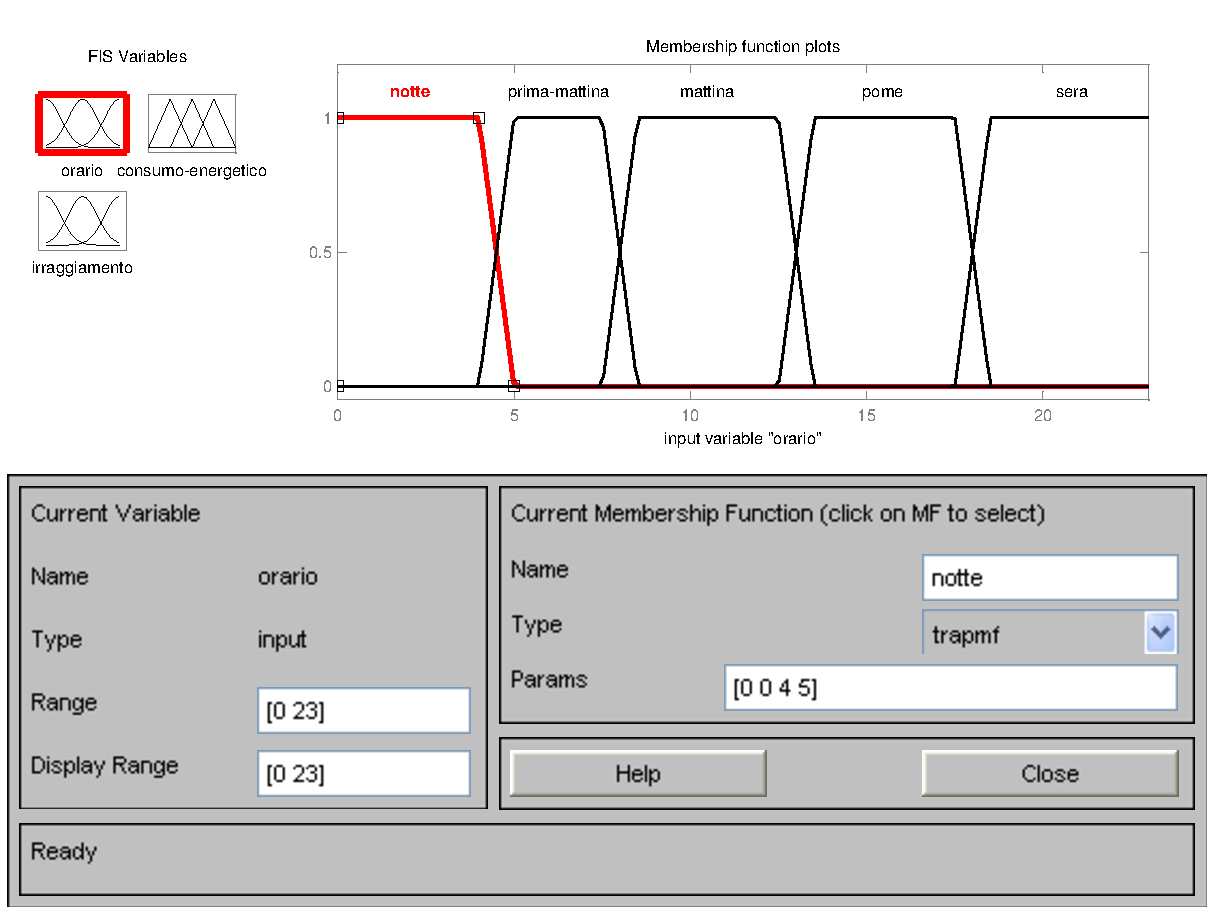
\includegraphics[scale=0.5]{images/fuzzy/variabile_orario.pdf}
  \caption{Variabile orario}
\end{figure}

Passando ora ad analizzare l'irraggiamento, attraverso lo studio dei dati forniti e del range di valori entro i quali si collocano, gli elementi lessicali sono quattro ({\em Basso, Medio, Alto, Molto Alto}) e le funzioni di appartenenza saranno:

\begin{figure}
  \centering
  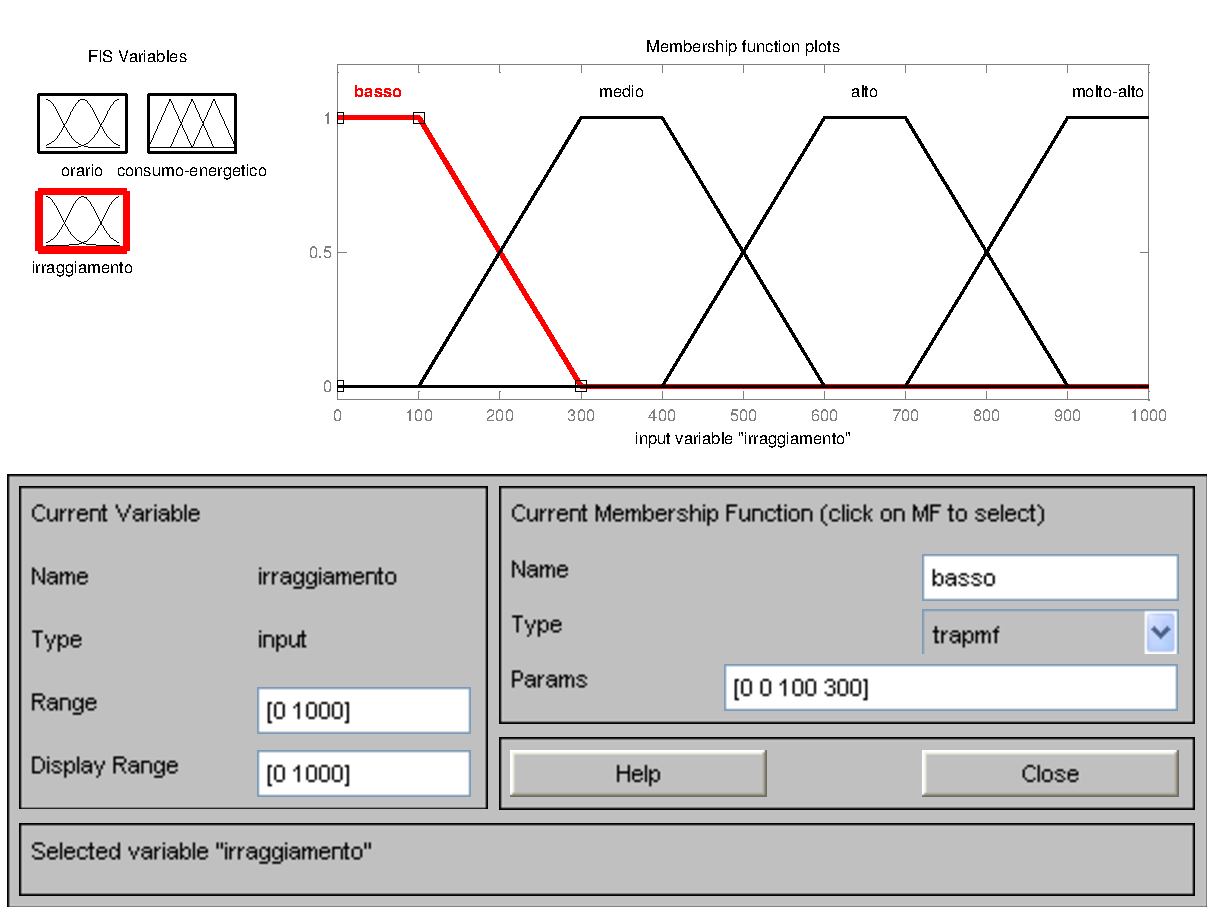
\includegraphics[scale=0.5]{images/fuzzy/variabile_irraggiamento.pdf}
  \caption{Variabile irraggiamento}
\end{figure}

Si possono ottenere con gli stessi ragionamenti risultati simili anche per la Luminosità:

\begin{figure}[htbp]
  \centering
  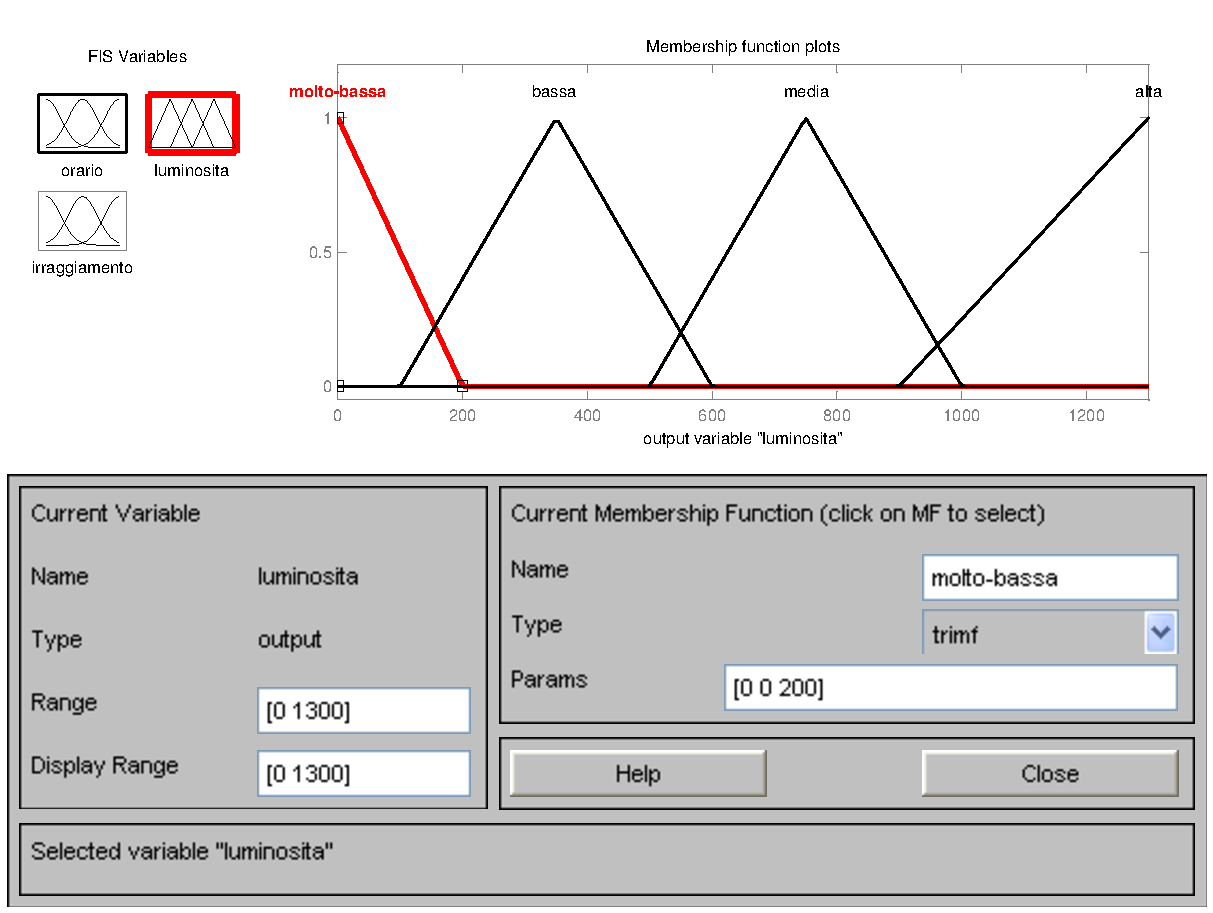
\includegraphics[scale=0.5]{images/fuzzy/variabile_luminosita.pdf}
  \caption{Variabile luminosità}
\end{figure}


\subsubsection{Definizione delle regole}
Non possedendo un'esperienza sufficiente nel campo dell'illuminazione per poter definire delle regole generali per il sistema fuzzy in esame, verranno estrapolate dai dati in nostro possesso le regole valide per il modello.

Nello specifico sono state ricavate le seguenti:

\begin{figure}[htbp]
  \centering
  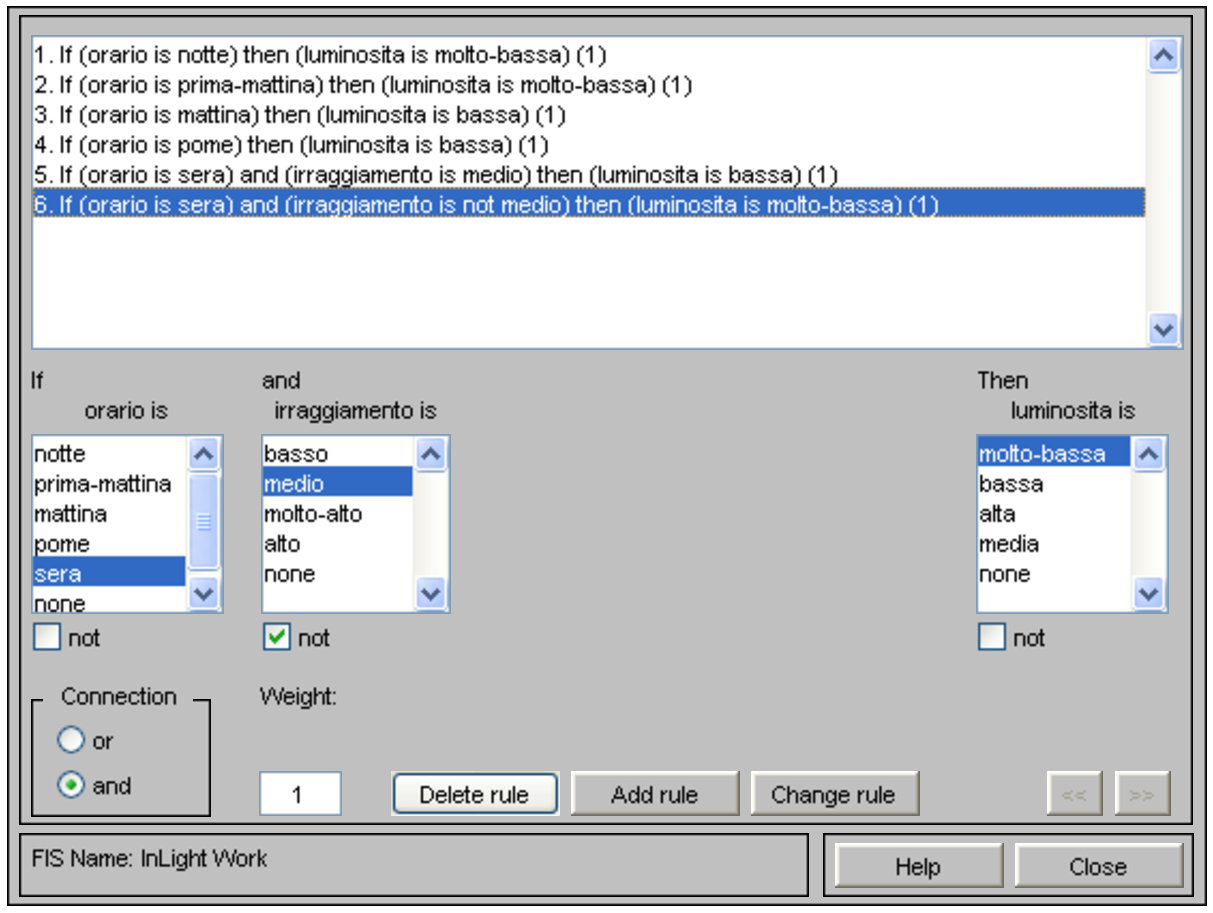
\includegraphics[scale=0.5]{images/fuzzy/regole_luminosita.pdf}
  \caption{Regole luminosità}
\end{figure}

A questo punto il FIS è completamente definita e si possono visualizzare le regole tramite il “Rule Viewer” e la curva tridimensionale che lega l'uscita ai due ingressi nel “Surface Viewer”:

\begin{figure}[htbp]
  \centering
  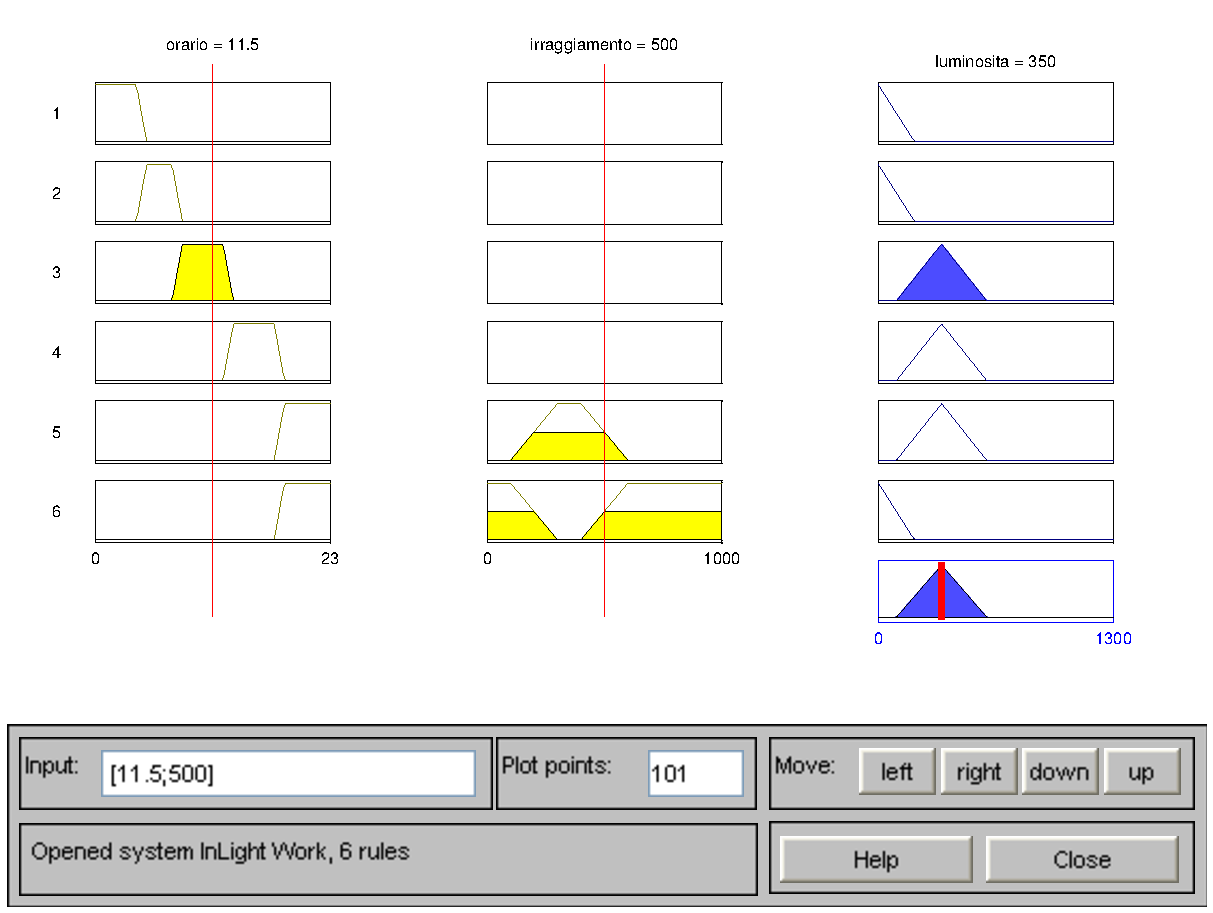
\includegraphics[scale=0.5]{images/fuzzy/regole_luminosita_rule_view.pdf}
  \caption{Regole luminosità rule view}
\end{figure}
\begin{figure}[htbp]
  \centering
  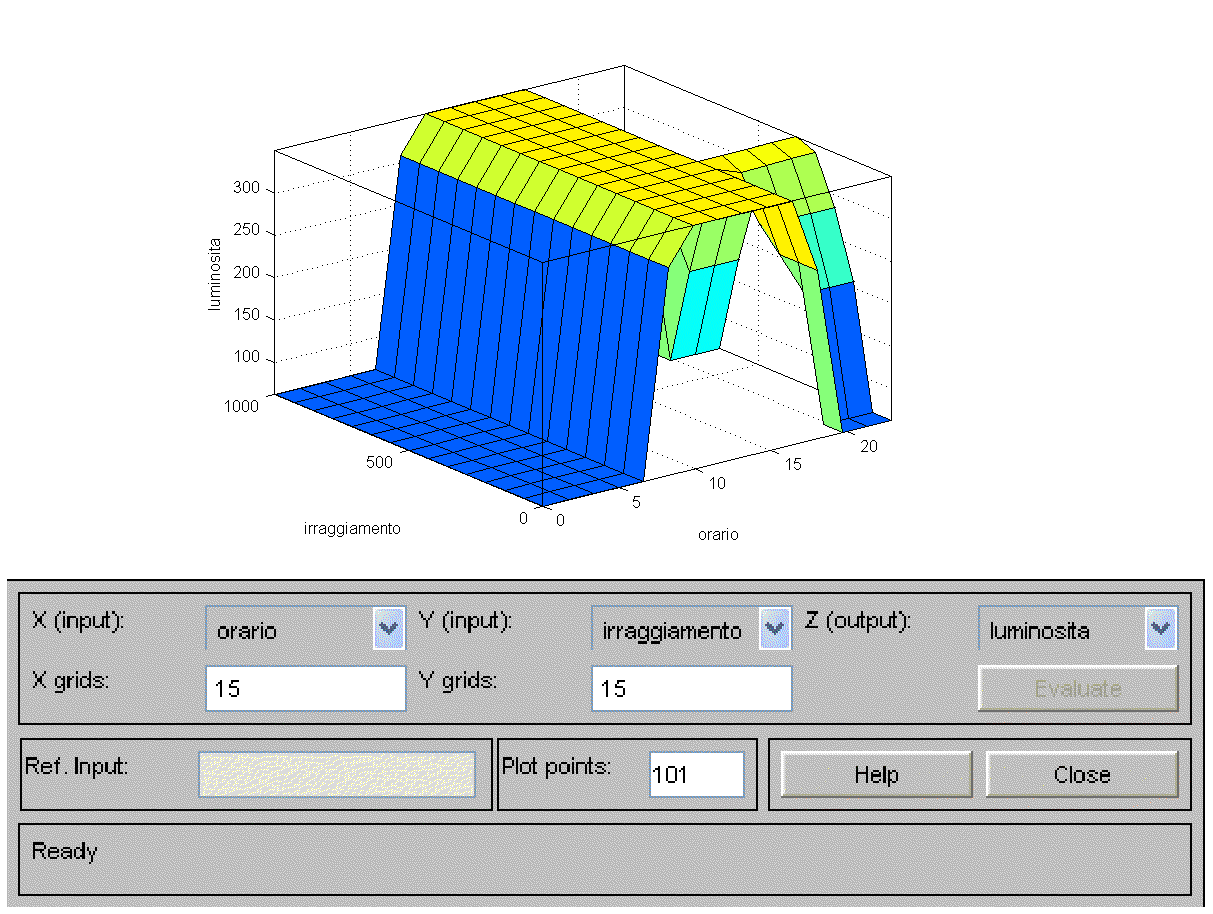
\includegraphics[scale=0.5]{images/fuzzy/regole_luminosita_surface_view.pdf}
  \caption{Regole luminosità surface view}
\end{figure}


\subsubsection{Manipolazione e studio dei risultati}
Una volta che il FIS è completamente definito deve essere valutato per testarne l'attendibilità.

Si utilizzerà perciò il comando Matlab “evalfis” assegnando in ingresso una coppia di vettori contenenti rispettivamente tutti i campioni forniti per ora e irraggiamento ( ovvero i due input del modello).

Il risultato fornito da evalfis sarà un vettore di valori crisp in cui l'i-esimo elemento rappresenta la Luminosità che il sistema fuzzy calcola per l'i-esima coppia in ingresso.

Si procede quindi alla fuzzificazione dei risultati forniti dal sistema e della luminosità presente nei dati. Confrontando i vettori si ottiene la percentuale di successi (hit), valore che può essere utilizzato come parametro prestazionale del sistema.

Per il caso in esame si ha una corrispondenza per 802 campioni, ovvero successo nell'80\% dei campioni.
\begin{table}
  \caption{Risultati}
  \centering
	\begin{tabular}{lr}
		\toprule
      \# di Entry & $1005$ \\
			\# di Hit   & $802$ \\
		\midrule
			& $80\%$ \\
		\bottomrule
	\end{tabular}
\end{table}


\subsubsection{Energia - Feriali}
Inseriamo, per completezza, i risultati finali ottenuti per le funzioni di appartenenza per la variabile d'uscita Consumo Energetico:
\begin{figure}[htbp]
  \centering
  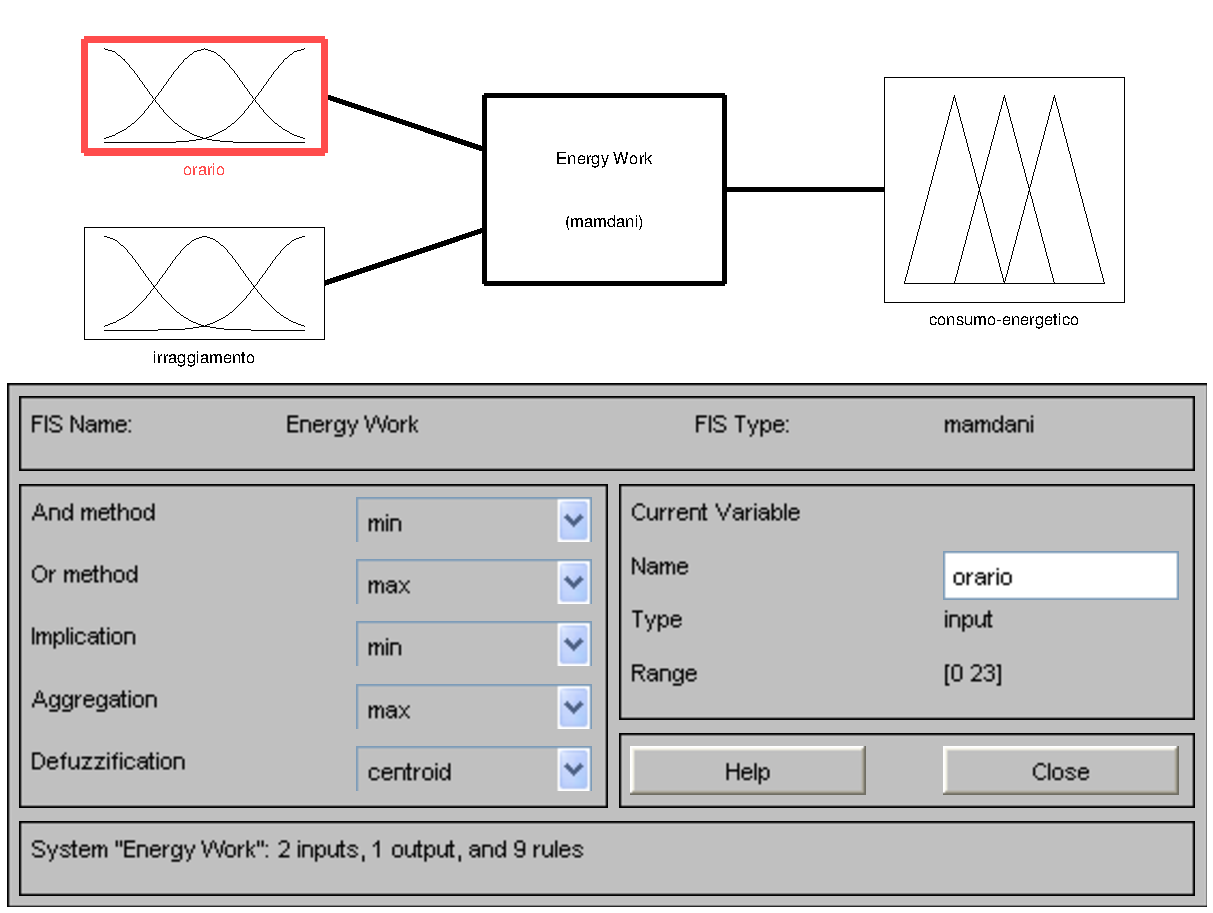
\includegraphics[scale=0.5]{images/fuzzy/modello_fuzzy.pdf}
  \caption{Modello fuzzy}
\end{figure}

\begin{figure}[htbp]
  \centering
  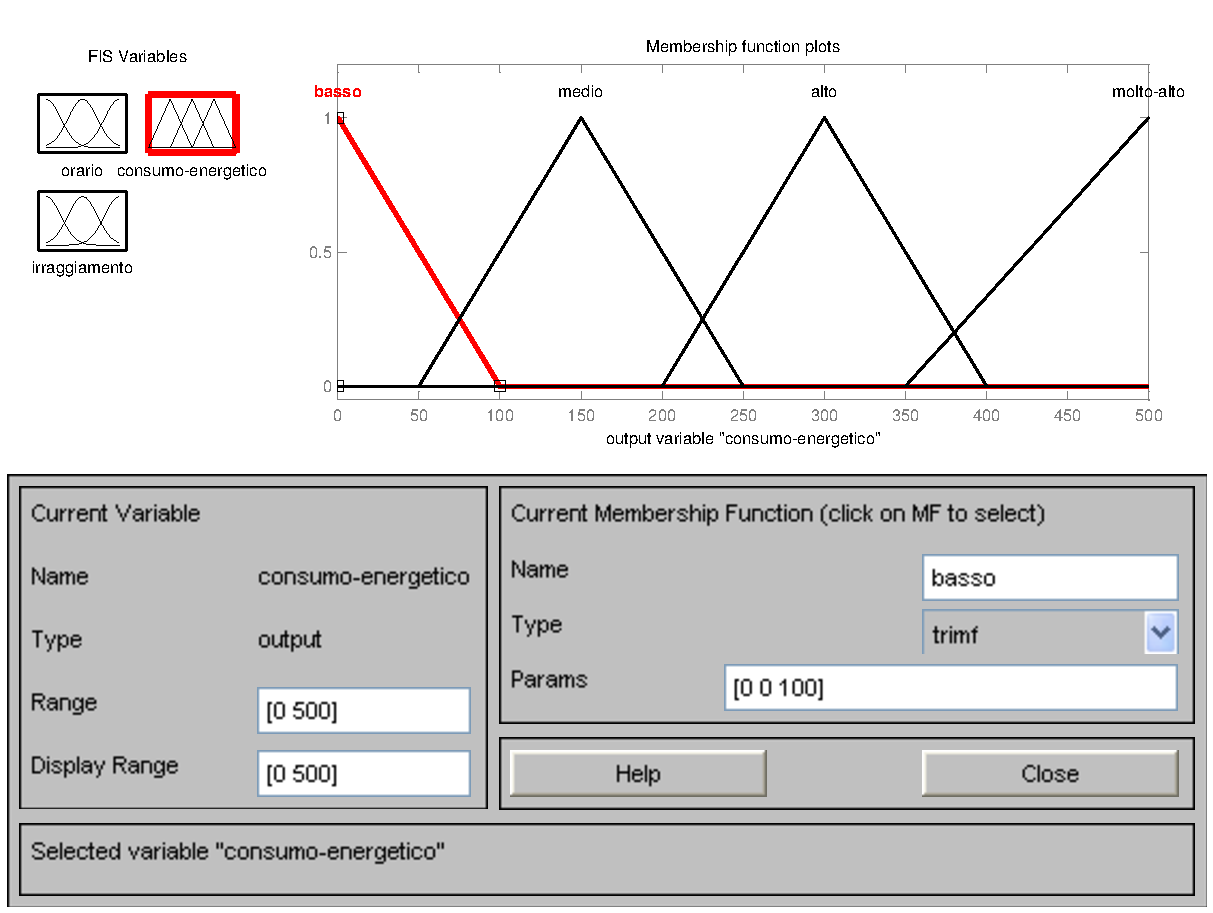
\includegraphics[scale=0.5]{images/fuzzy/variabile_consumo_energetico.pdf}
  \caption{Variabile consumo energetico}
\end{figure}

Per lo studio dell'energia nei giorni feriali, effettuando gli stessi ragionamenti e seguendo la procedura appena descritta otteniamo:
\begin{figure}[htbp]
  \centering
  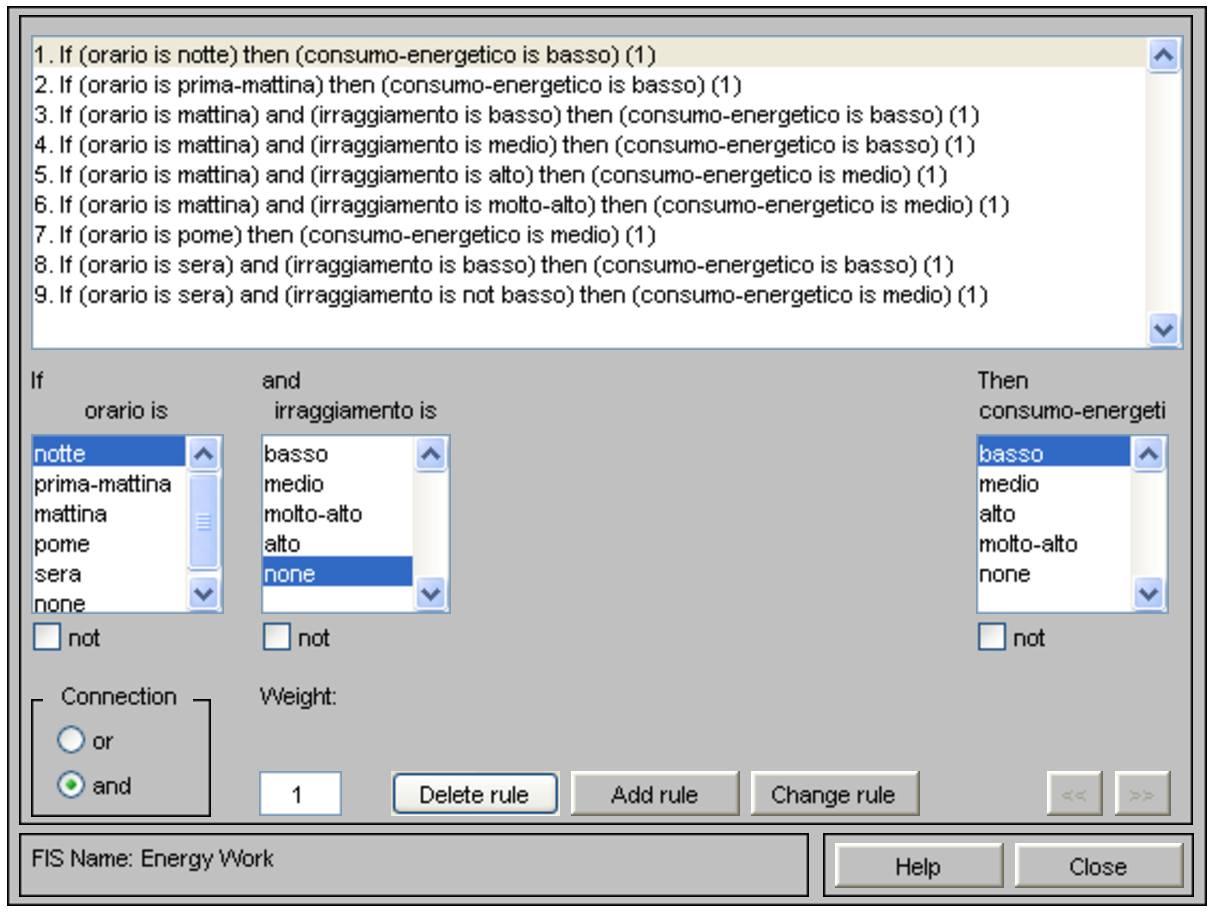
\includegraphics[scale=0.5]{images/fuzzy/energia_feriali_regole.pdf}
  \caption{Energia feriali: regole}
\end{figure}

\begin{figure}[htbp]
  \centering
  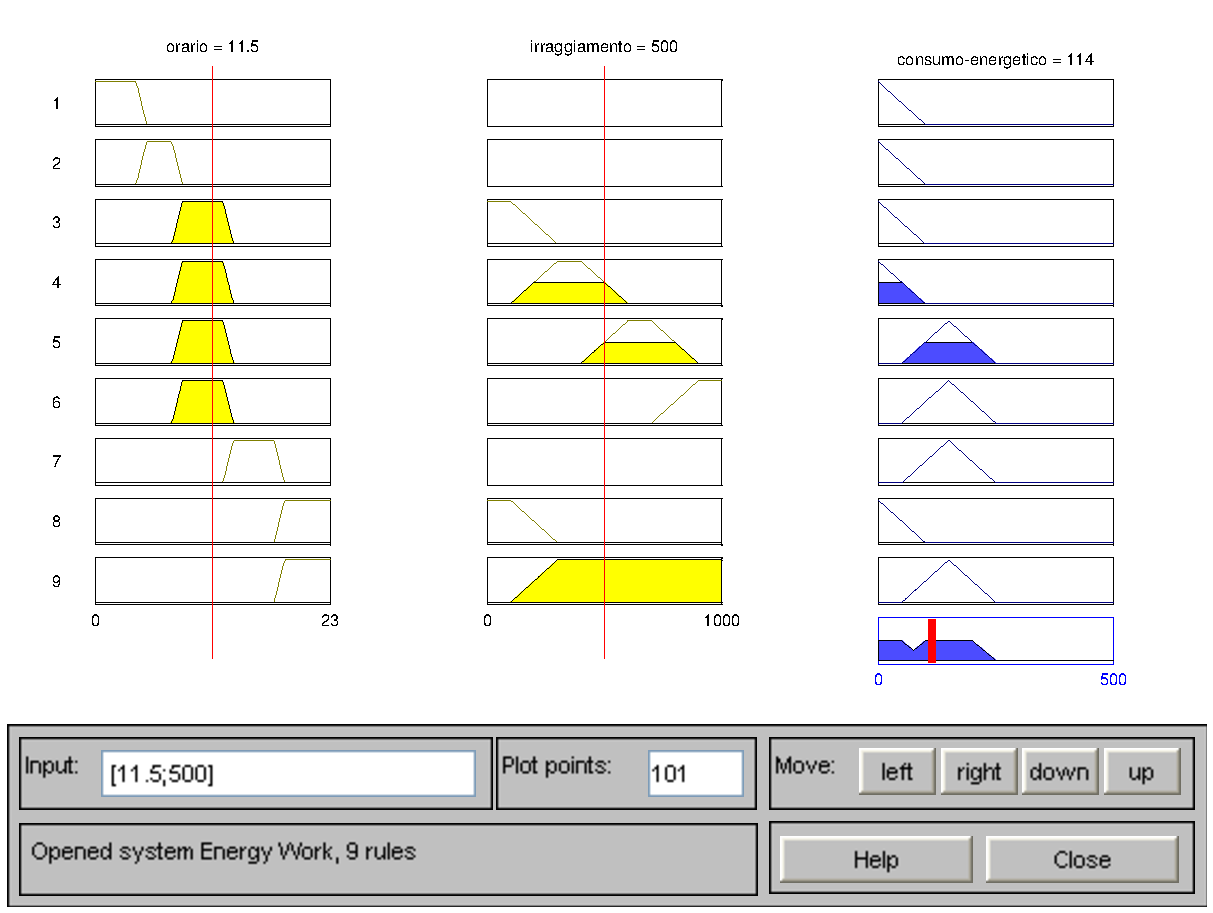
\includegraphics[scale=0.5]{images/fuzzy/energia_feriali_rule_view.pdf}
  \caption{Energia feriali: rule view}
\end{figure}

\begin{figure}[htbp]
  \centering
  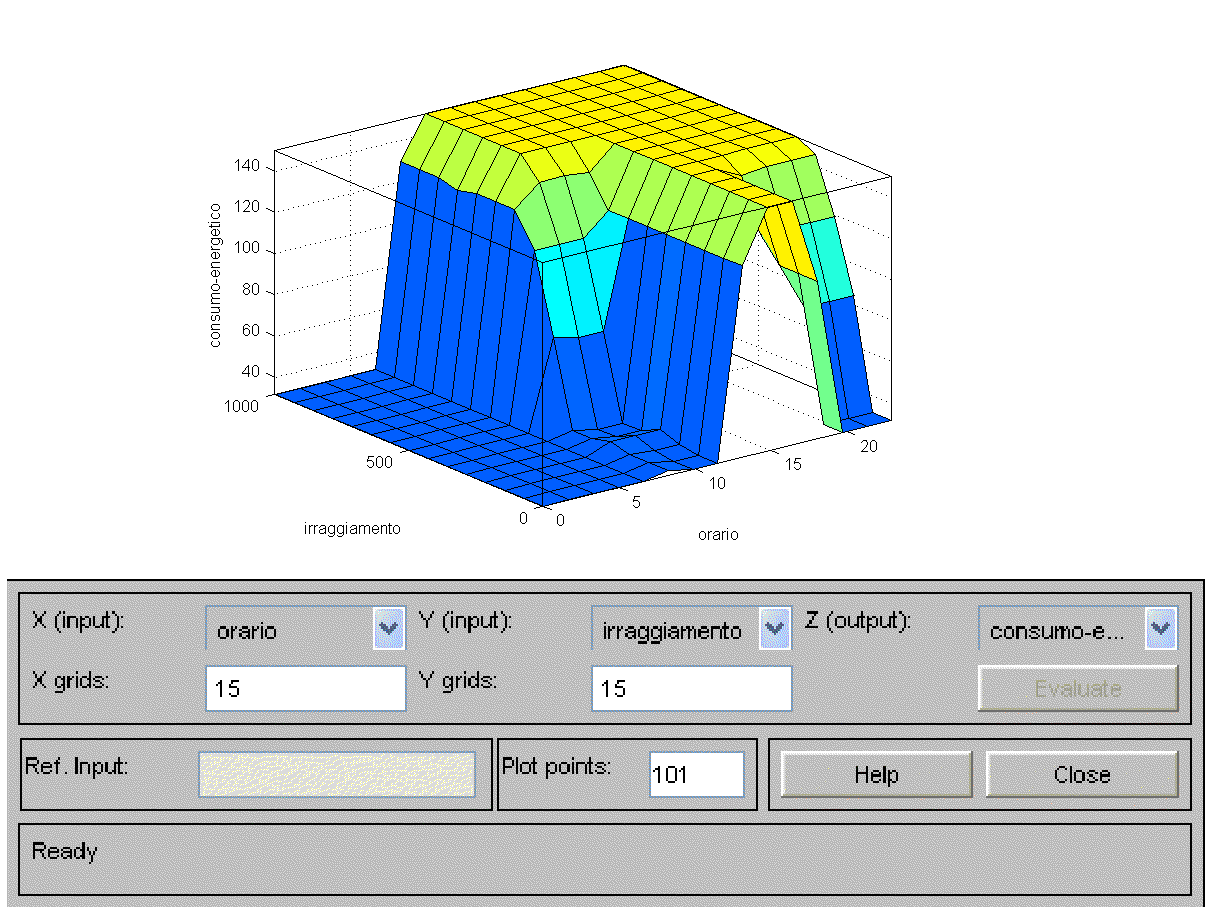
\includegraphics[scale=0.5]{images/fuzzy/energia_feriali_surface_view.pdf}
  \caption{Energia feriali: surface view}
\end{figure}

\begin{table}
  \caption{Risultati}
  \centering
	\begin{tabular}{lr}
		\toprule
      \# di Entry & $ 1005 $ \\
			\# di Hit   & $ 781 $ \\
		\midrule
			& $ 78\% $ \\
		\bottomrule
	\end{tabular}
\end{table}


\subsubsection{Luminosità - Festivi}

\begin{figure}[htbp]
  \centering
  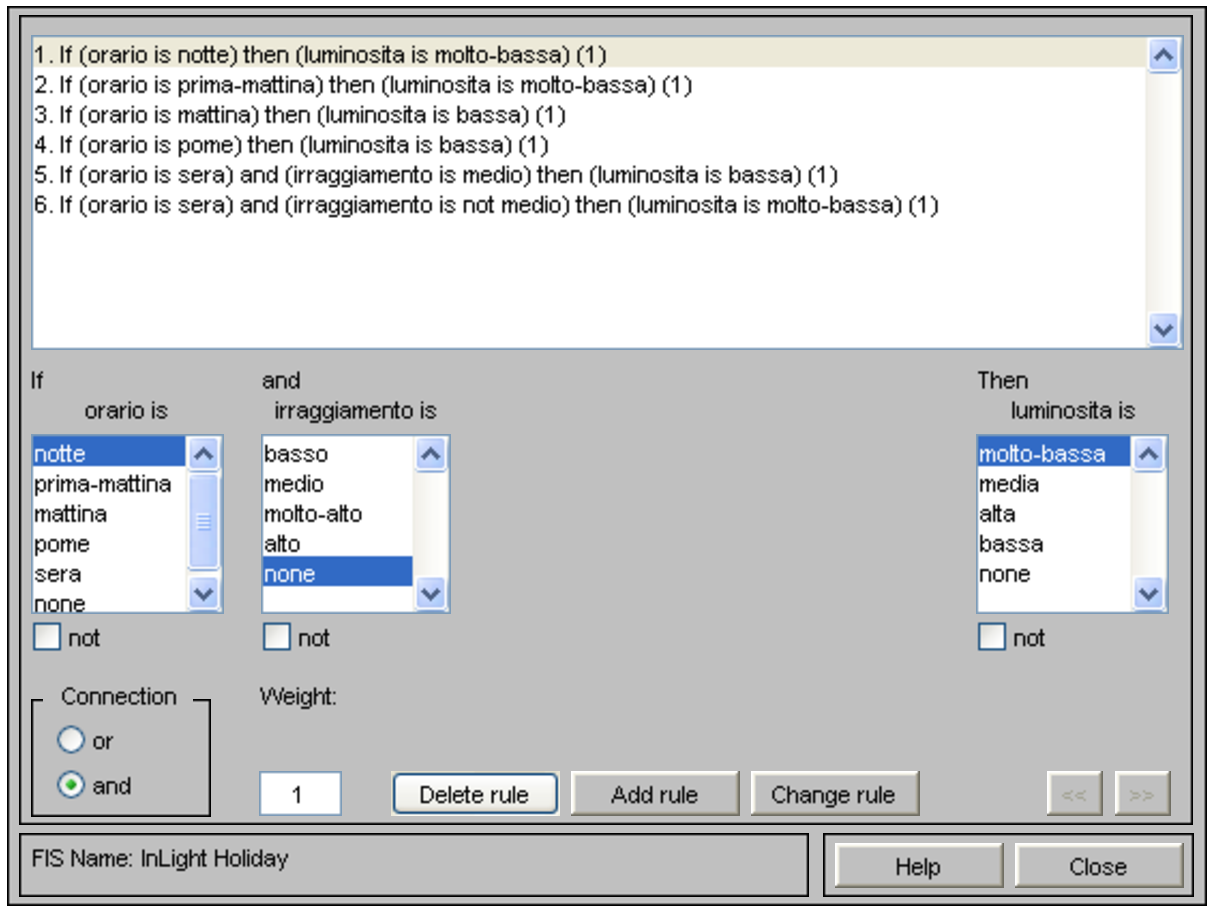
\includegraphics[scale=0.5]{images/fuzzy/luminosita_festivi_regole.pdf}
  \caption{Luminosità festivi: regole}
\end{figure}

\begin{figure}[htbp]
  \centering
  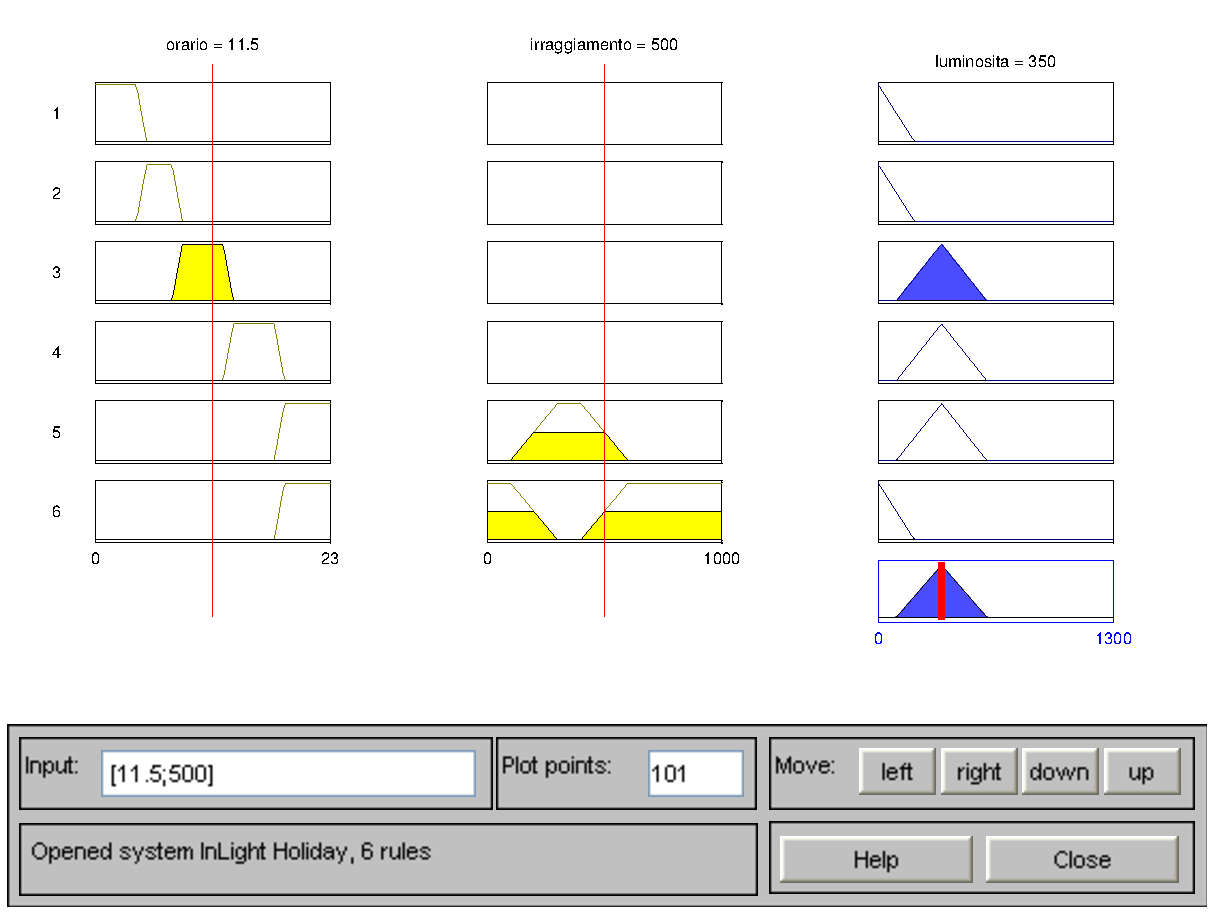
\includegraphics[scale=0.5]{images/fuzzy/luminosita_festivi_rule_view.pdf}
  \caption{Luminosità festivi: rule view}
\end{figure}

\begin{figure}[htbp]
  \centering
  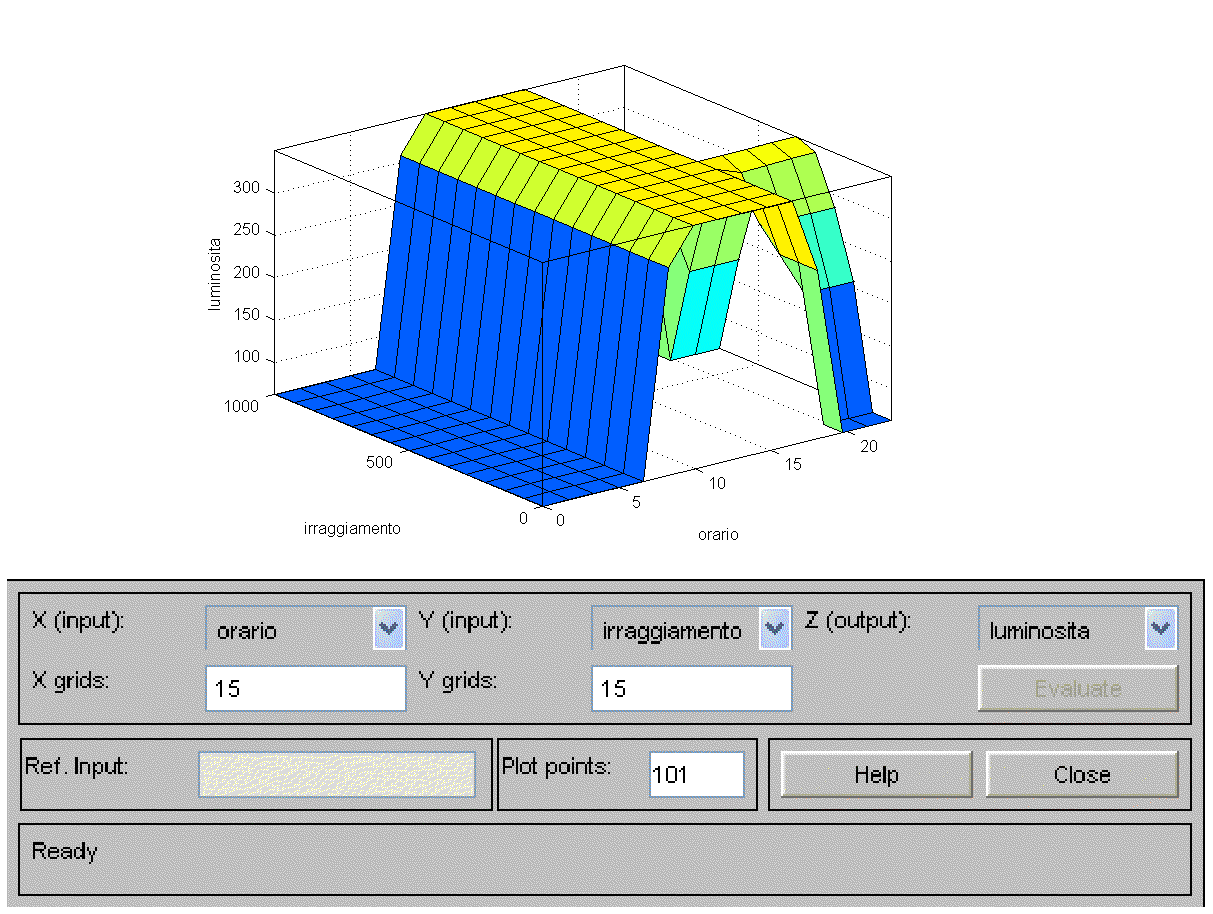
\includegraphics[scale=0.5]{images/fuzzy/luminosita_festivi_surface_view.pdf}
  \caption{Luminosità festivi: surface view}
\end{figure}

\begin{table}
  \caption{Risultati}
  \centering
	\begin{tabular}{lr}
		\toprule
      \# di Entry & $ 528 $ \\
			\# di Hit   & $ 436 $ \\
		\midrule
			& $ 83\% $ \\
		\bottomrule
	\end{tabular}
\end{table}


\subsubsection{Energia - Festivi}

\begin{figure}[htbp]
  \centering
  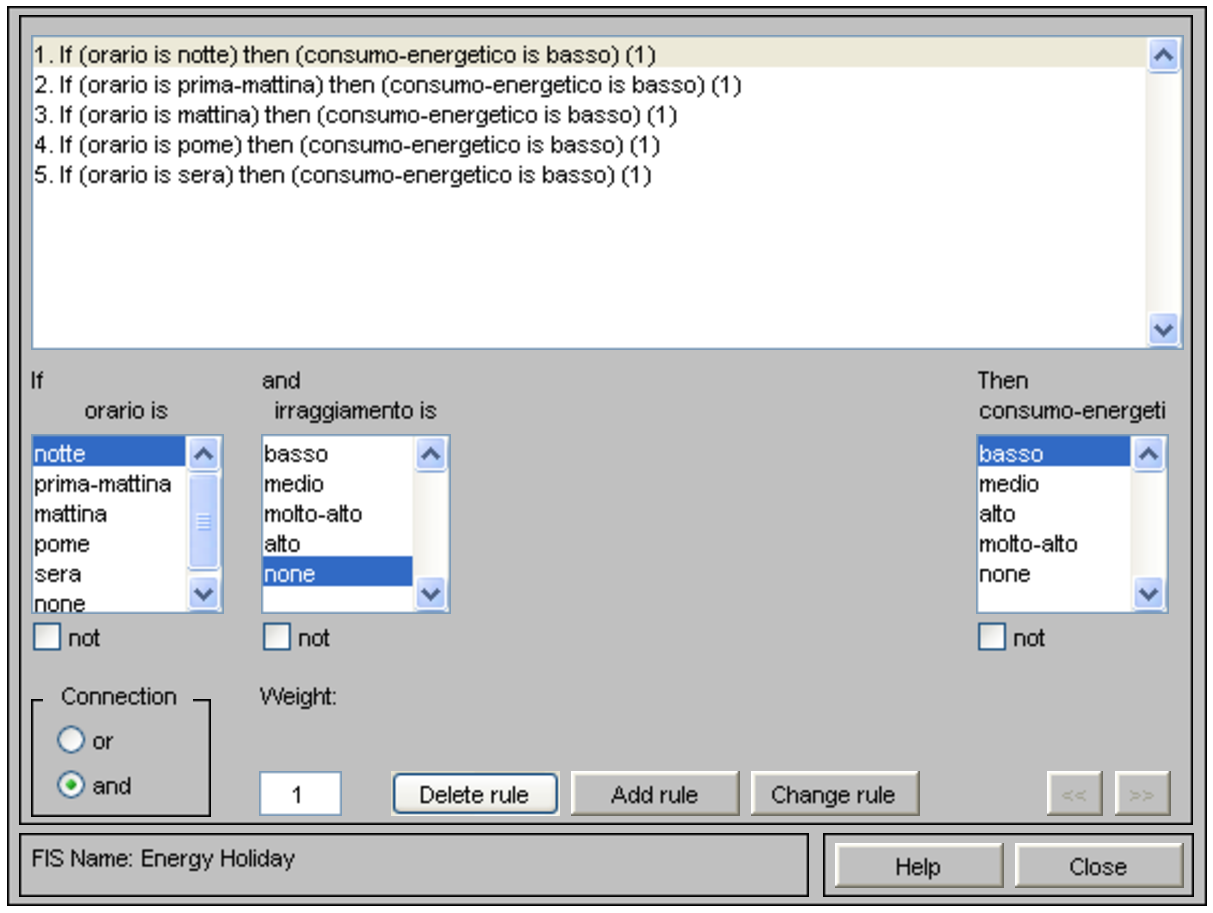
\includegraphics[scale=0.5]{images/fuzzy/energia_festivi_regole.pdf}
  \caption{Energia festivi: regole}
\end{figure}

\begin{figure}[htbp]
  \centering
  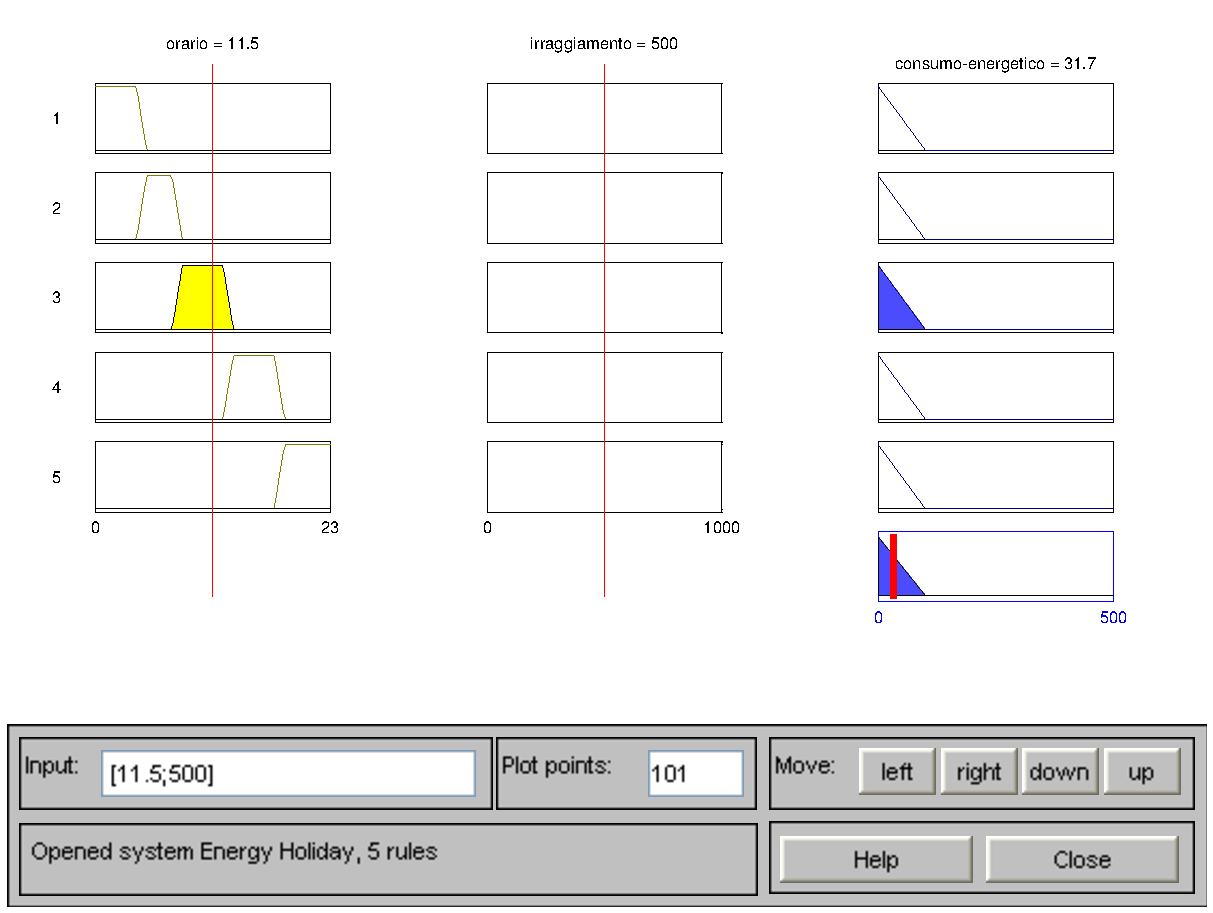
\includegraphics[scale=0.5]{images/fuzzy/energia_festivi_rule_view.pdf}
  \caption{Energia festivi: rule view}
\end{figure}

\begin{figure}[htbp]
  \centering
  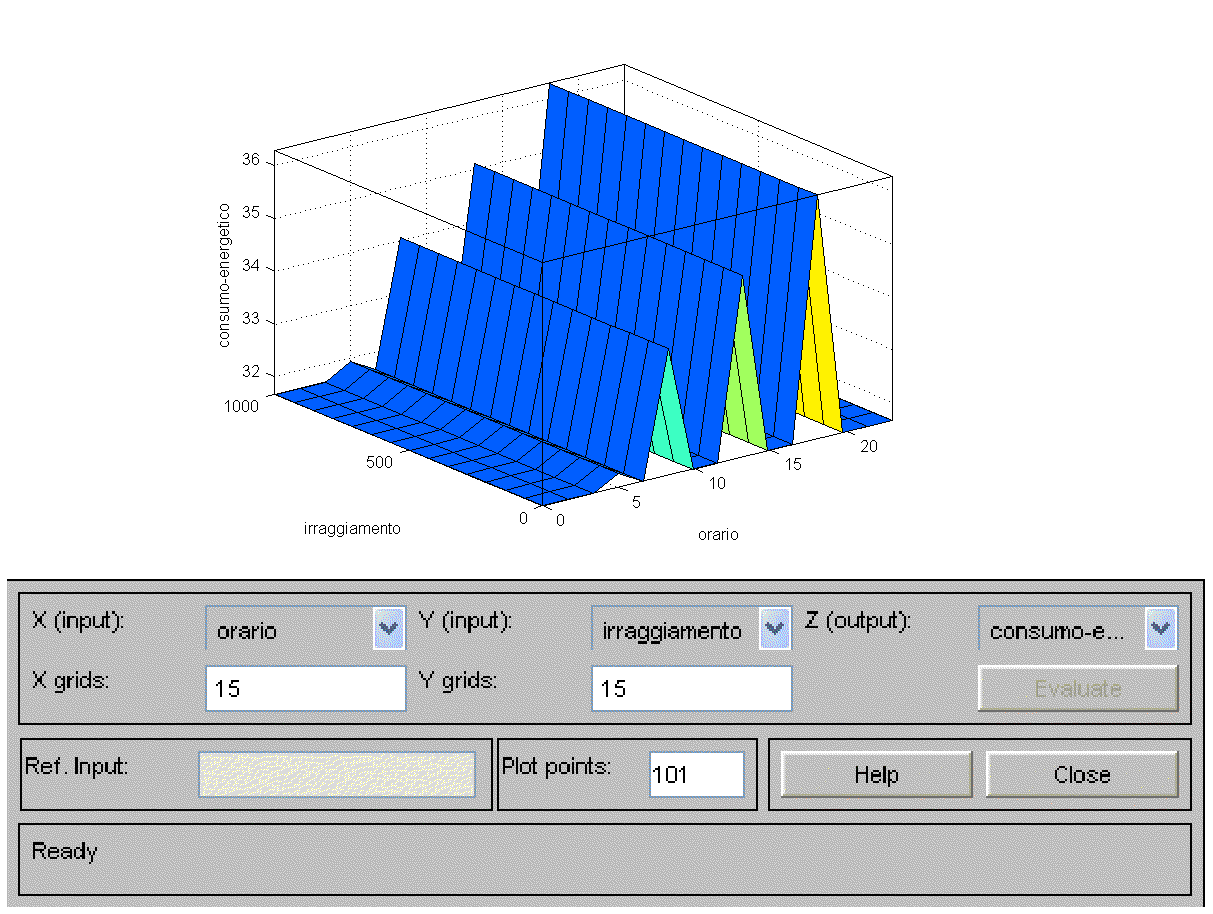
\includegraphics[scale=0.5]{images/fuzzy/energia_festivi_surface_view.pdf}
  \caption{Energia festivi: surface view}
\end{figure}

\begin{table}
  \caption{Risultati}
  \centering
	\begin{tabular}{lr}
		\toprule
      \# di Entry & $ 528 $ \\
			\# di Hit   & $ 491 $ \\
		\midrule
			& $ 93\% $ \\
		\bottomrule
	\end{tabular}
\end{table}


\section{Modelli di predizione}
\subsection{Rete neurale con elementi di ritardo}

Una rete neurale con elementi di ritardo presenta un uscita dipendente, oltre che dagli ingressi attuali e dagli stati della rete, anche dagli ingressi passati (ottenuti tramite ritardi o delays) ed uscite passate (ottenute tramite feedbacks).

Scopo di queste reti è quello di usare valori passati di una serie temporale per predire quelli futuri: se indichiamo con x(t) il vettore di input all’istante t, e con y(t) il vettore di output al medesimo istante, abbiamo che y(t) sarà funzione degli ultimi N vettori risultato del sistema e degli ultimi N vettori di input.

%% FIXME: riscrivere usando sintassi latex standard
$$
y(t)=f(y(t\lyxmathsym{\textminus}1),y(t\lyxmathsym{\textminus}2),...,y(t\lyxmathsym{\textminus}N),x(t\lyxmathsym{\textminus}1),x(t\lyxmathsym{\textminus}2),...,x(t\lyxmathsym{\textminus}N))
$$

Anche in questo caso, ad ogni passo dell'addestramento, il vettore di output generato dal sistema viene confrontato con il corrispondente vettore obiettivo, e a seconda della differenza vengono opportunamente aggiornati i pesi dei neuroni che compongono gli strati nascosti e lo strato di uscita, fino ad ottenere un livello di generalizzazione soddisfacente.

L'approccio usato per la modellizzazione di questa rete è del tutto analogo a quello usato con la rete neurale statica prima enunciata, l'unica differenza è che questa volta, per agevolare ulteriormente l'apprendimento della rete neurale, è stato decisio di creare una rete per ogni tipo di uscita; sono quindi state modellizzate due reti distinte: una per l'energia stimata ed una per la luminosità interna all'edificio.

Infine anche in questo caso poteva essere utilizzato direttamente il tool proposto da Matlab (nntstool), usufruendo quindi della GUI proposta, ma per gli stessi inconvenienti già esposti, è stato deciso di creare uno script analogo al caso precedente per ricavare questo tipo di rete in modo automatico.

Il tipo di rete che tratteremo in questa sezione è quella mostrata nella figura seguente:\\

\vspace{20px}
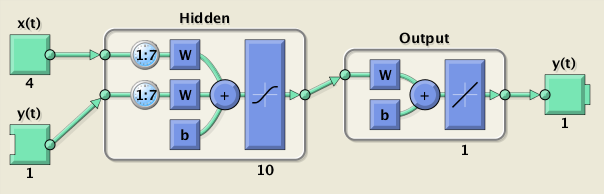
\includegraphics[scale=0.5]{images/timeseries/energia/net.png}
\captionof{figure}[One figure]{Rete neurale esogena autoregressiva}
\vspace{20px}

\subsubsection{Suddivisione dei dati}

Il primo passo per la creazione delle due reti è stato quello di suddividere i dati riportati nel file csv, creato da conform.rb, in due divesi files, ottenendo dunque un totale di quattro files.

I primi due conterranno gli ingressi delle reti ( i due files sono identici ), i secondi due invece conterranno una diversa colonna di uscita: energia consumata e luminosità interna rispettivamente.


\paragraph{Script energy.rb}

Questo semplice script ruby elabora il file conformData.csv ed estrapola la colonna di uscita inerente all'energia consumata, creando dunque due ulteriori files ( inputEnergy e targetEnergy ) i quali riporteranno al loro interno rispettivamente gli inputs e le relative uscite inerenti all'energia consumata all'interno dello stabile.

\inputminted[linenos=true,fontsize=\footnotesize]{ruby}{../../data/time\ series/energy.rb}
\captionof{listing}{data/time series/energy.rb}


\paragraph{Script inlight.rb}

Lo stesso procedimento è stato eseguito anche per la luminosità interna all'edificio.

\inputminted[linenos=true,fontsize=\footnotesize]{ruby}{../../data/time\ series/inlight.rb}
\captionof{listing}{data/time series/inlight.rb}


\subsubsection{Rircerca della migliore rete neurale}
Nell'ottica di automatizzare il processo di creazione della rete, è stata definita sia una funzione apposita il cui scopo è la ricerca di una rete neurale con elementi di ritardo considerata ottima, sia uno script per la visualizzazione dei risultati ottenuti.

\paragraph{Funzione searchBestTimeSeries}
Scopo di tale funzione è quello di ricercare, se esiste, una rete caratterizzata da parametri ottimali o in alternativa di restituire la rete che ha presentato il miglior apprendimento: quindi con il minor MSE riscontrato ed il più alto coefficiente di regressione.

L'approccio seguito è del tutto simile a quello visto per la modellizzazione di una rete statica; vengono definiti:

\begin{itemize}
  \item Valore minimo e massimo per i delays sia per gli ingressi che per l'uscita.
  \item Numero minimo e massimo di neuroni nascosti
  \item Numero di addestramenti per ogni configurazione di rete
  \item Goals che si desiderano raggiungere, in altre parole le caratteristiche che una rete deve presentare per essere classificata come ottima (in termini di MSE e coefficiente di retta di regressione).
  \item I tre valori cardini di ogni rete neurale: percentuali di test, validation e train.
\end{itemize}

La funzione, partendo dai valori di defaults, modella una rete neurale di tipo esogena auto-regressive (NARX), la allena, la valida ed infine la prova.

Ad ogni passo della funzione vengono fatte variare le variabili sopra enunciate in modo da confrontare tra loro le performances di diverse reti.

Una volta ottenuti i risultati in termini di MSE e retta di regressione ( entrambi inerenti alla fase di test in quanto quella che assicura la generalizzazione ), vengono confrontati con quelli precedentemente salvati e, se migliori, registrati.

Occorre infine dire che anche in questo caso la funzione di addestramento utilizzata è quella standard di backpropagation di Levenberg-Marquardt (trainlm).

\inputminted[linenos=true,fontsize=\footnotesize]{matlab}{../../src/time\ series/functions/searchBestTimeSeries.m}
\captionof{listing}{src/time\ series/functions/searchBestTimeSeries.m}


\paragraph{Script netts.m}
Scopo di questo script matlab è quello di invocare la funzione appena enunciata e di mostrarne i valori restituiti.

\inputminted[linenos=true,fontsize=\footnotesize]{matlab}{../../src/netts.m}
\captionof{listing}{src/netts.m}


\subsubsection{Risultati}

\paragraph{Energia consumata}
\hspace{10px} \\
\vspace{20px}
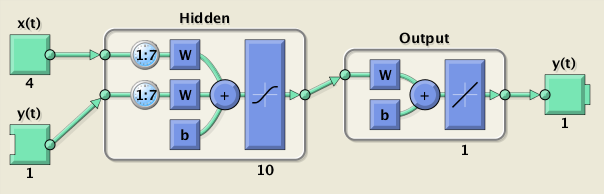
\includegraphics[scale=0.5]{images/timeseries/energia/net.png}
\captionof{figure}[One figure]{Rete usata}
\vspace{20px}

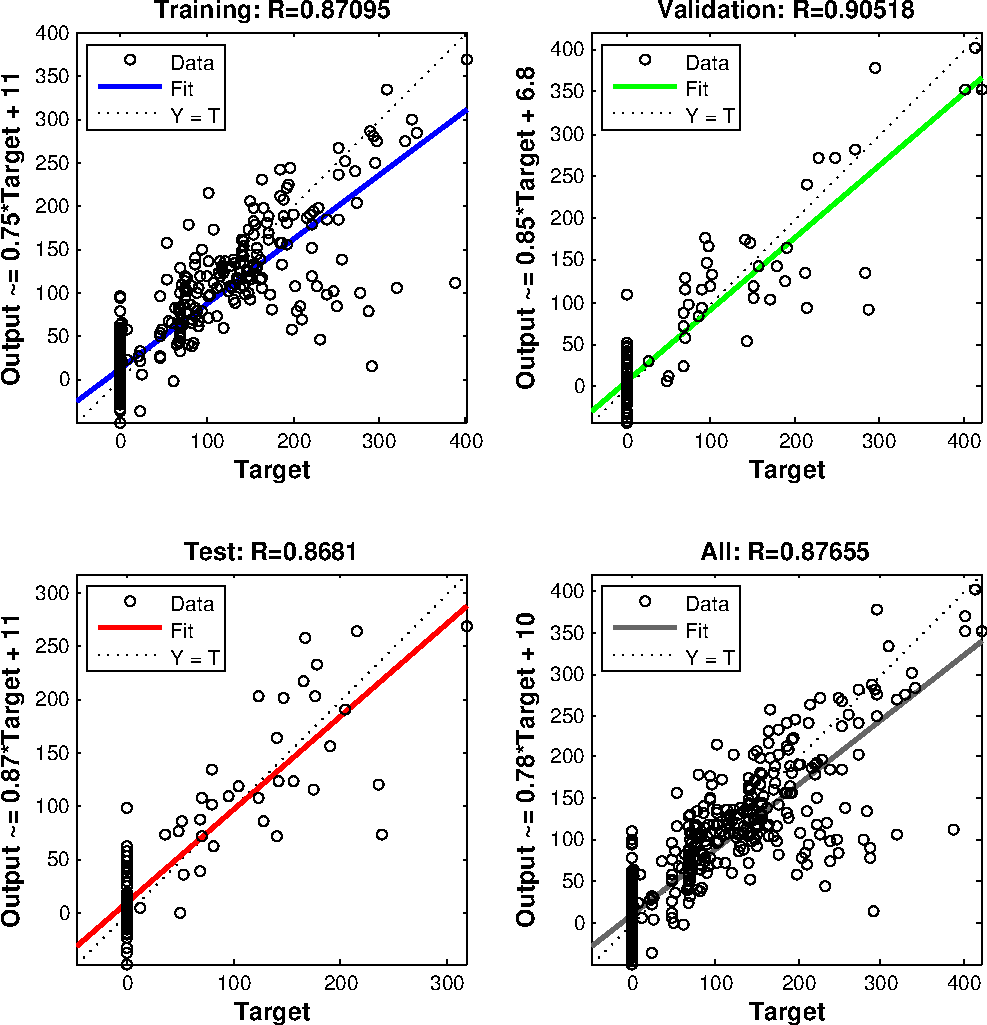
\includegraphics[scale=0.5]{images/timeseries/energia/regressions.pdf}
\captionof{figure}[One figure]{Retta di regressione}
\vspace{20px}

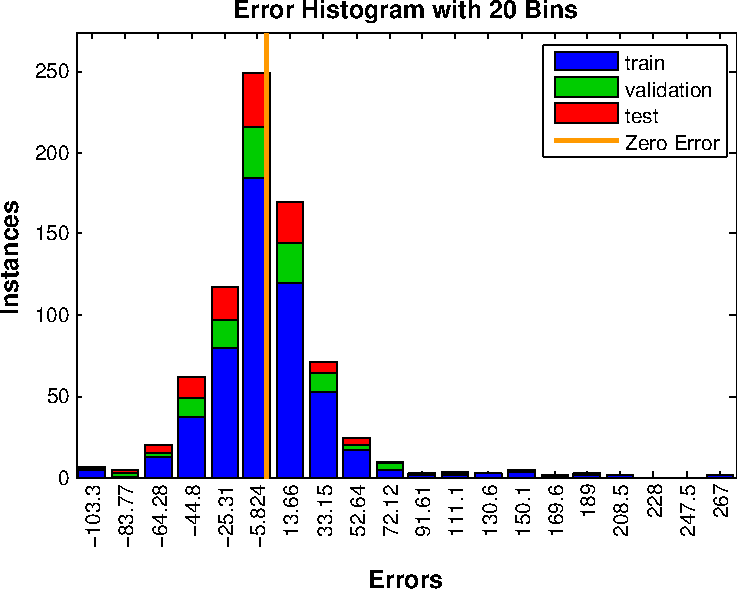
\includegraphics[scale=0.5]{images/timeseries/energia/histogram.pdf}
\captionof{figure}[One figure]{Istrogramma degli errori}
\vspace{20px}

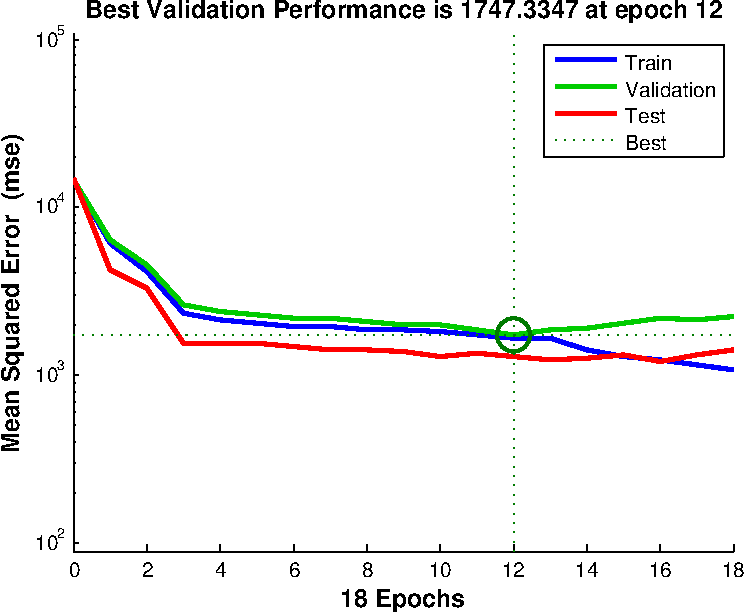
\includegraphics[scale=0.5]{images/timeseries/energia/performances.pdf}
\captionof{figure}[One figure]{Performance}
\vspace{20px}

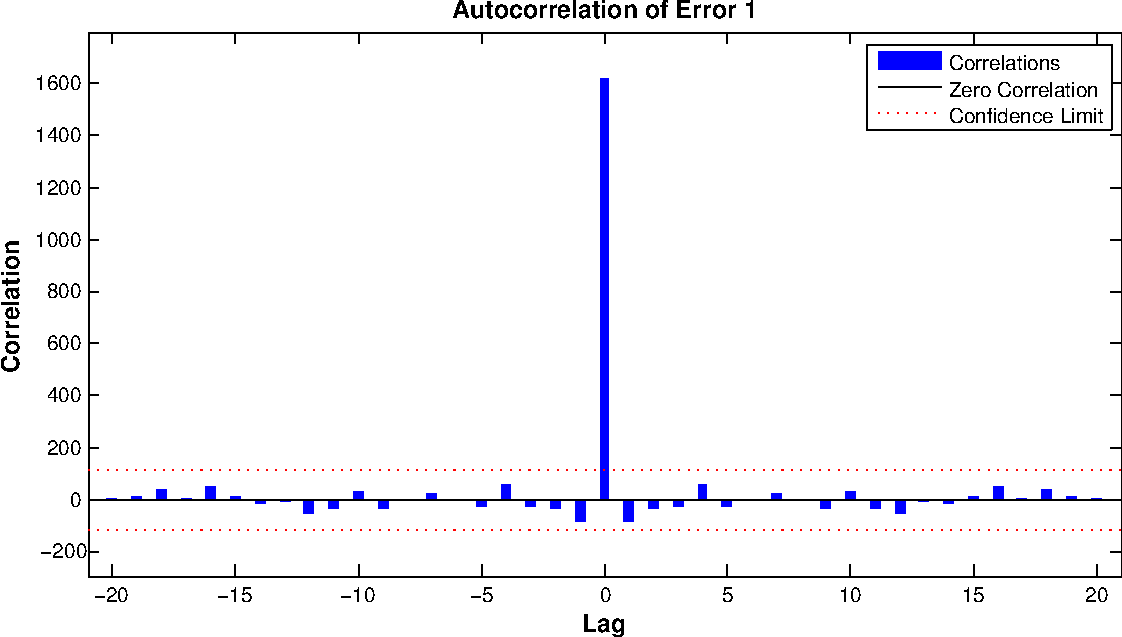
\includegraphics[scale=0.5]{images/timeseries/energia/autocorrelations.pdf}
\captionof{figure}[One figure]{Autocorrelazione errore}
\vspace{20px}

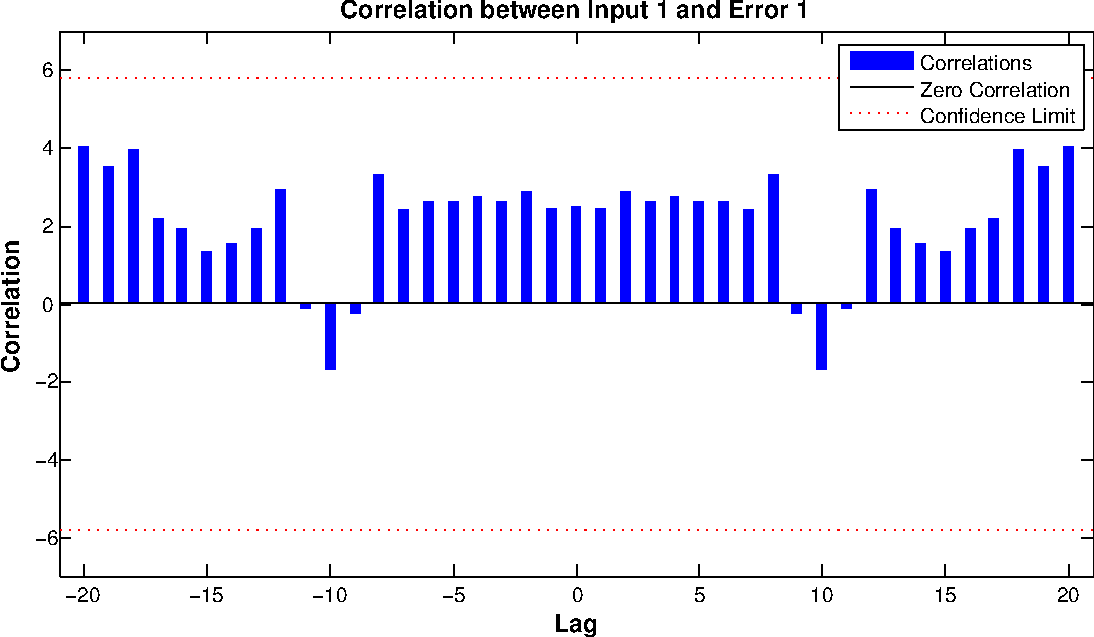
\includegraphics[scale=0.5]{images/timeseries/energia/correlations.pdf}
\captionof{figure}[One figure]{Correlazione tra input e output}
\vspace{20px}


\paragraph{Luce interna}
\hspace{10px} \\
\vspace{20px}
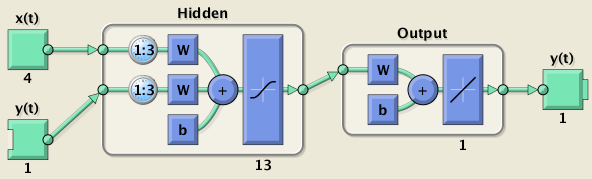
\includegraphics[scale=0.5]{images/timeseries/inlight/net.png}
\captionof{figure}[One figure]{Rete usata}
\vspace{20px}

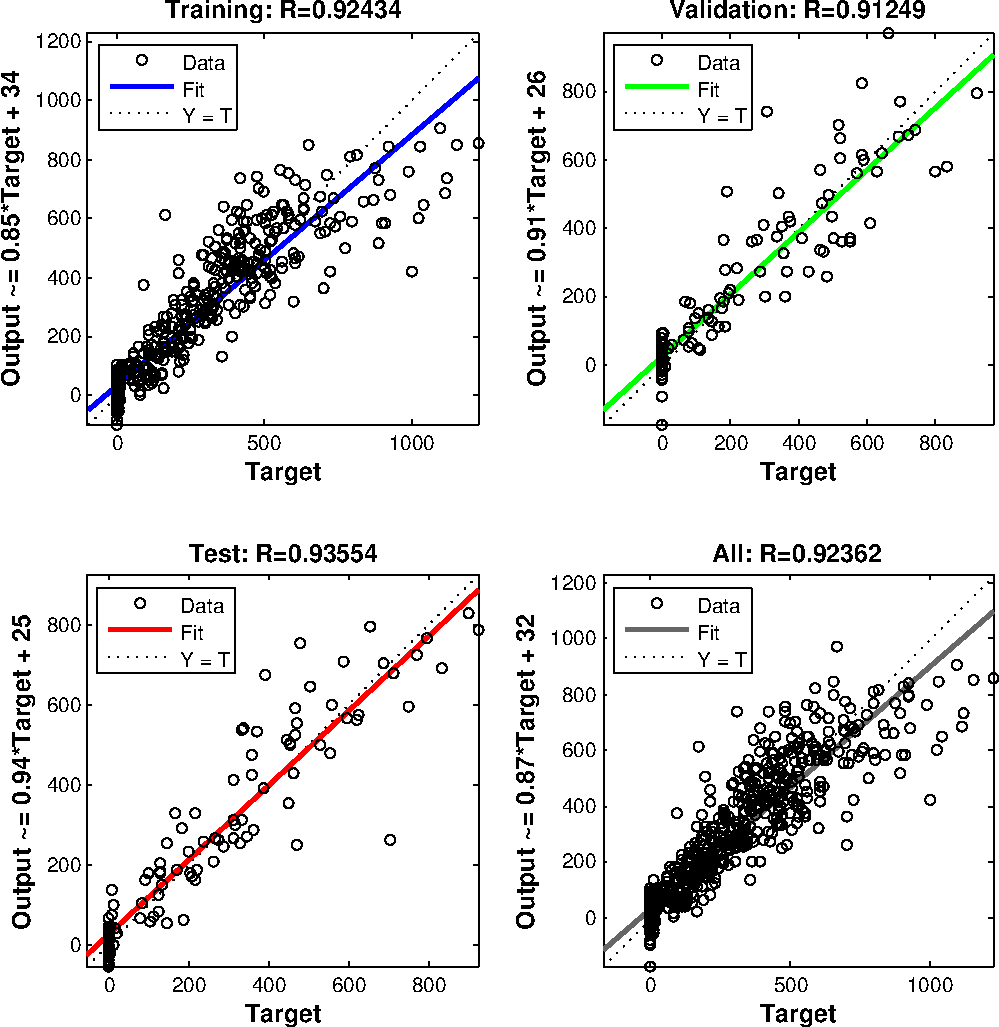
\includegraphics[scale=0.5]{images/timeseries/inlight/regressions.pdf}
\captionof{figure}[One figure]{Retta di regressione}
\vspace{20px}

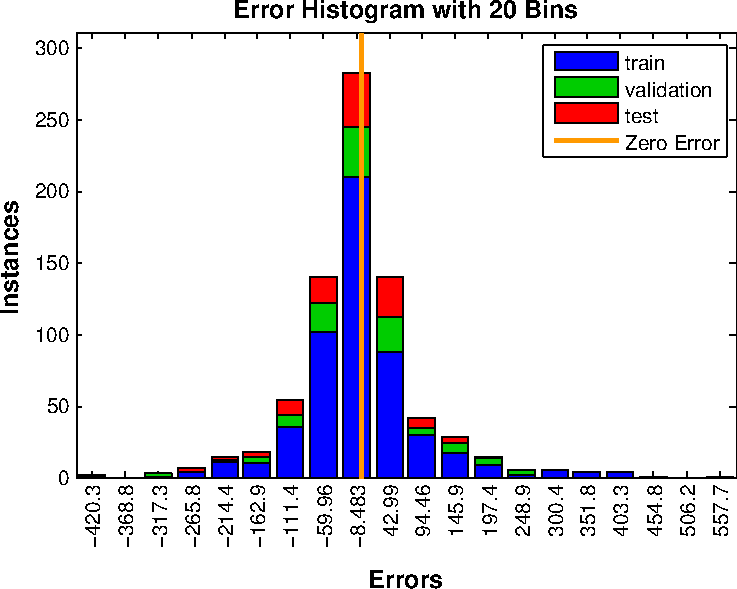
\includegraphics[scale=0.5]{images/timeseries/inlight/histogram.pdf}
\captionof{figure}[One figure]{Istrogramma degli errori}
\vspace{20px}

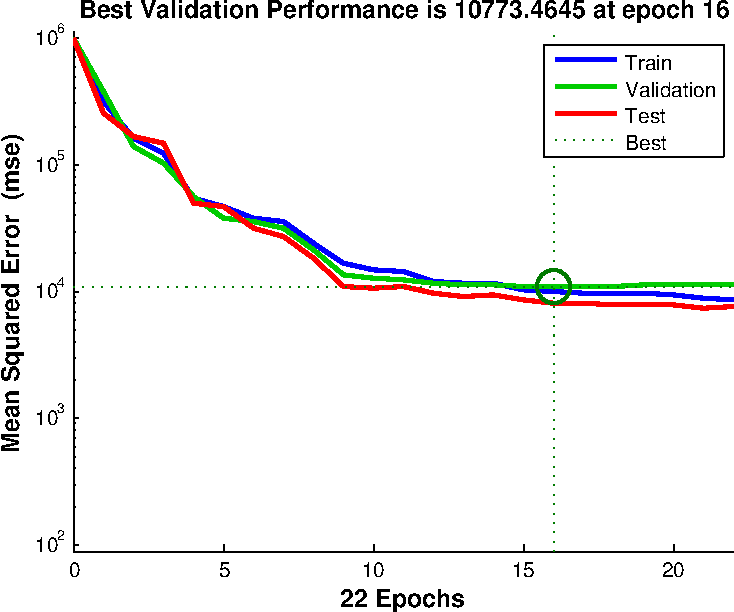
\includegraphics[scale=0.5]{images/timeseries/inlight/performances.pdf}
\captionof{figure}[One figure]{Performance}
\vspace{20px}

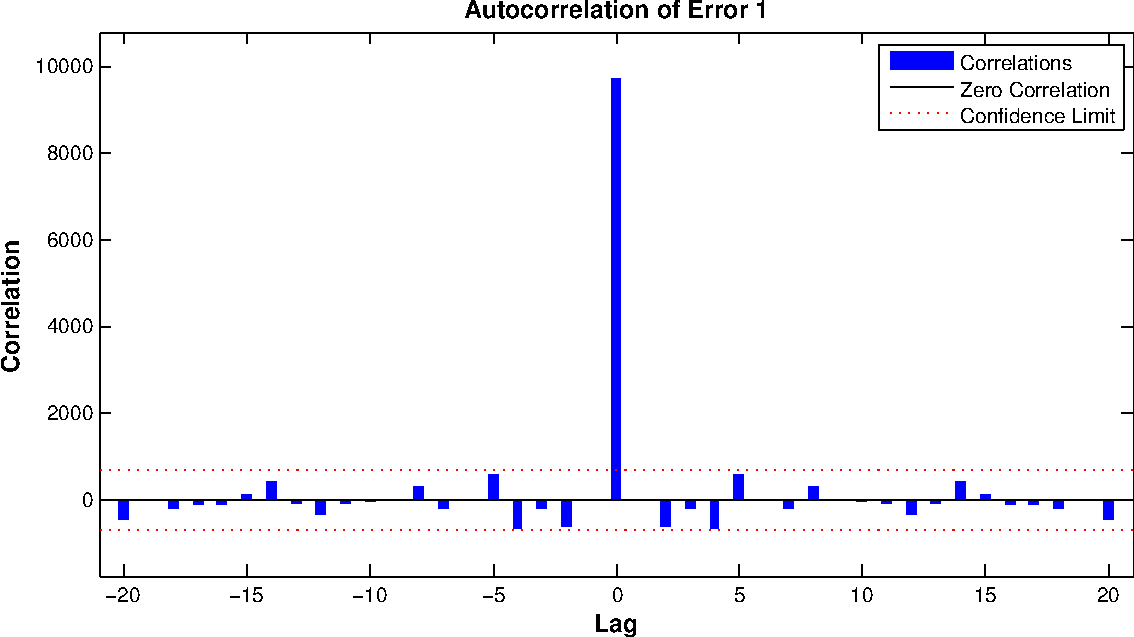
\includegraphics[scale=0.5]{images/timeseries/inlight/autocorrelations.pdf}
\captionof{figure}[One figure]{Autocorrelazione errore}
\vspace{20px}

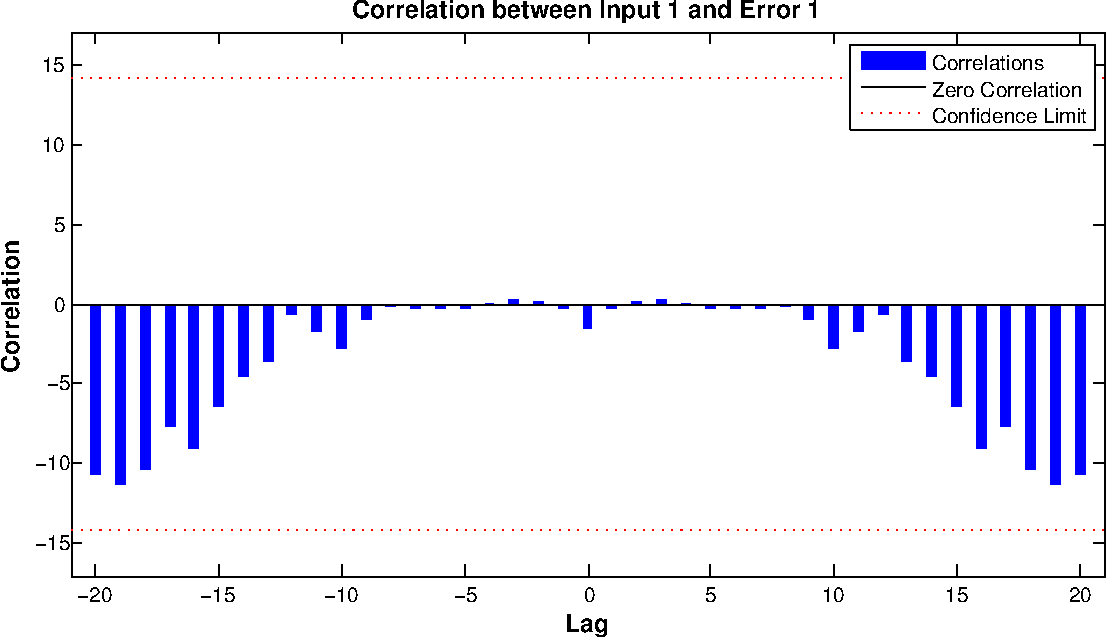
\includegraphics[scale=0.5]{images/timeseries/inlight/correlations.pdf}
\captionof{figure}[One figure]{Correlazione tra input e output}
\vspace{20px}

\clearpage


\section{A.N.F.I.S.}            % FIXME: ma a cosa appartiete? fitting o prediction?
\subsection{A.N.F.I.S.}
Finora abbiamo supposto di conoscere a fondo ogni caratteristica del problema che ci viene posto (ci siamo comportati da “esperti”) , supponiamo adesso invece di essere in presenza del seguente scenario:

\begin{itemize}
  \item E' disponibile una collezione di dati (inputs/outputs) da usare per la modellizzazione della rete.
  \item Le funzioni di appartenenza, ed i loro parametri, non sono state arbitrariamente fissate dall'interpretazione dell'esperto.
  \item Non è presente una struttura predeterminata del modello basata sulle caratteristiche delle variabili del sistema.
\end{itemize}

In uno scenario come questo vengono utilizzate quelle che vengono chiamate reti adattive, ovvero reti multistrato dove ogni nodo esegue una particolare funzione sui segnali ricevuti in ingresso, e dove ognuno di essi può contenere (in linea generale) dei parametri.\\

\vspace{20px}
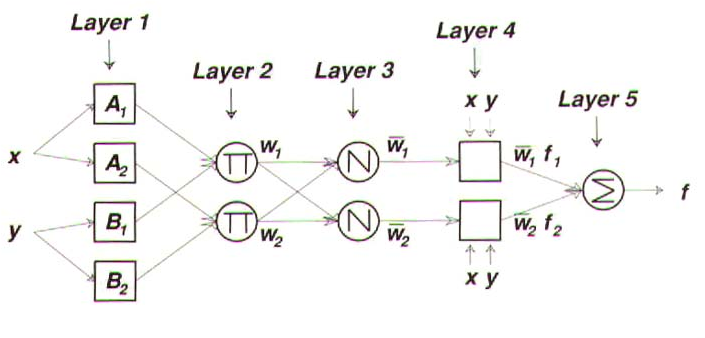
\includegraphics[scale=0.5]{images/anfis/adaptive.png}
\captionof{figure}[One figure]{I nodi quadrati contengono parametri ed eseguono funzioni, gli altri eseguono solo funzioni}
\vspace{20px}

Con il termine A.N.F.I.S. (adaptive network based fuzzy inference system) si indica una classe di reti adattive funzionalmente equivalenti al sistema di inferenza fuzzy; in particolare utilizzando reti di tipo A.N.F.I.S. è possibile costruire una rete del tutto equivalente al sistema di inferenza Takagi-Sugeno-Kang.

Anche in questo caso Matlab mette a disposizione un semplice tool (anfisedit) con il quale è possibile definire una rete A.N.F.I.S.; in questo caso però deve essere già prevista una suddivisione dei dati da presentare al tool, nei casi precedenti invece tale suddivione (training, test e validation) era fatta dai tools in modo automatico.

Nello specifico i dati usati per la fase di training dovrebbero rappresentare in modo completo la realtà così che le funzioni di appartenenza possano essere fissate adeguatamente; anche in questo caso vengono utilizzati due ulteriori files che contengono sia i dati per la fase di checking (analoga alla fase di validation) sia per la fase di tests.

I dati sono stati suddivisi nei tre files a mano (per quanto appena detto) usando le percentuali canoniche: 70\% training, 15\% checking e 15\% tests.

Il tool anfis supporta solamente sistemi di tipo Sugeno, aventi le seguenti condizioni:

\begin{itemize}
  \item Il sistema Sugeno deve essere di grado uno o zero.
  \item Deve presentare una singola uscita ottenuta mediante il metodo di defuzzificazione della media pesata.
  \item Tutte le funzioni di appartenenza dell'uscita devono essere dello stesso tipo e devono essere lineari o costanti.
  \item Diverse regole non possono condividere la stessa funzione di appartenenza di uscita; quindi il numero di funzioni membro delle uscita deve essere uguale al numero di regole.
  \item Possiede peso unitario per ogni regola % FIXME: * Have unity weight for each rule (che minchia vuol dire???)
\end{itemize}

Durante la fase di setup è inoltre richiesto che l'utente specifichi sia quante funzioni di appartenenza andranno usate per gli ingressi ed il tipo (trapezoidali, triangolari etc.), sia il tipo di funzione per l'uscita (lineare o costante).

Bisogna poi indicare il tipo di ottimizzazione usata durante la fase di training ( backpropagation o hybrid), il numero di epoche ed il “training Error Tolerance” per impostare i criteri di stop della fase di allenamento: il processo di training si fermerà dunque quando si raggiunge il massimo numero di epoche o il goal (espresso mediante la error tolerance).


\subsubsection{Ricerca della rete migliore}

Anche in questo caso si è deciso di automatizzare il processo di generazione delle reti; in particolare le variabili su cui la funzione lavora sono principalmente due:
\begin{itemize}
  \item Il numero di funzioni di appartenenza di cui ogni ingresso è composto.
  \item Il numero di epoche della fase di addestramento.
\end{itemize}

Tale funzione (searchBestAnfis) una volta inizializzate le variabili sopra citate, crea la rete e ne misura le performances, ovvero ne calcola l'MSE (mean square error) usando i dati di test.

Se il risultato ottenuto supera il goal (fissato a 20) esce immediatamente; altrimenti controlla se tale MSE è minore di quello della migliore rete trovata fino a questo momento; in caso positivo salva i parametri attuali, altrimenti prosegue semplicemente.

In questo caso sono state modellate tre diverse reti: una per i giorni festivi la cui uscita è la luminosità interna all'edificio e due per i giorni feriali (luminosità ed energia consumata); non è stata creata la rete per l'energia consumata per i giorni festivi in quanto dopo un analisi dei dati si è riscontrato che l'output è praticamente sempre nullo.

Infine le funzioni di appartenenza degli ingressi hanno una forma fissa a “campana” (la forma non è una variabile della funzione), e l'uscita è lineare.


\paragraph{Funzione searchBestAnfis}
La funzione che esegue quanto appena detto è la seguente:

\inputminted[linenos=true,fontsize=\footnotesize]{matlab}{../../src/anfis/functions/searchBestAnfis.m}
\captionof{listing}{src/anfis/functions/searchBestAnfis.m}


\paragraph{Script netanfis}
Lo scopo di tale script è quello di lanciare la funzione sopra enunciata e di resituirne i valori.

\inputminted[linenos=true,fontsize=\footnotesize]{matlab}{../../src/netanfis.m}
\captionof{listing}{src/netanfis.m}

Tale script fa uso della funzione testplot creata appositamente per visualizzare i risultati.


\paragraph{Funzione testplot}
Questa funzione stampa a schermo le uscite di una rete dato un vettore di ingressi.
\inputminted[linenos=true,fontsize=\footnotesize]{matlab}{../../src/anfis/functions/testplot.m}
\captionof{listing}{src/anfis/functions/testplot.m}


\subsubsection{Risultati}

%% FIXME: Qui servirebbero un po piu di figure come ad esempio l'andamento degli errori! L'unica cosa è che avendo svolto questo punto con il tool si ottengono usando anfisedit

Sono sotto riportati i grafici (ottenuti nelle tre reti relativi ai casi di tests) che mostrano le relazioni output/target.\\
\vspace{20px}
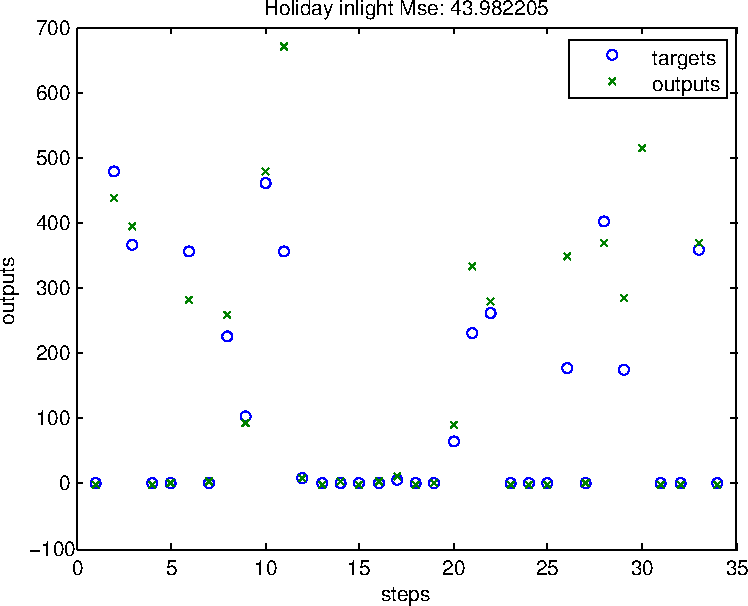
\includegraphics[scale=0.5]{images/anfis/holiday/inlight.pdf}
\captionof{figure}[One figure]{Luce interna nei giorni festivi}
\vspace{20px}

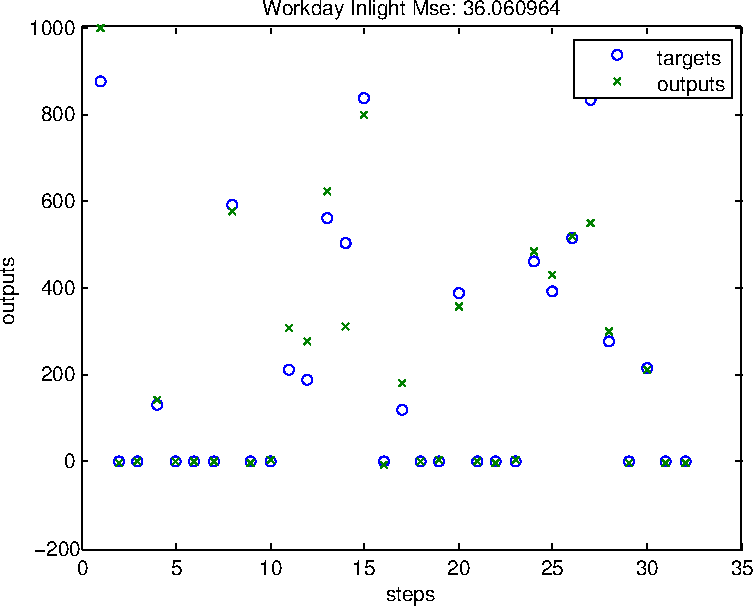
\includegraphics[scale=0.5]{images/anfis/workday/inlight.pdf}
\captionof{figure}[One figure]{Luce interna nei giorni feriali}
\vspace{20px}

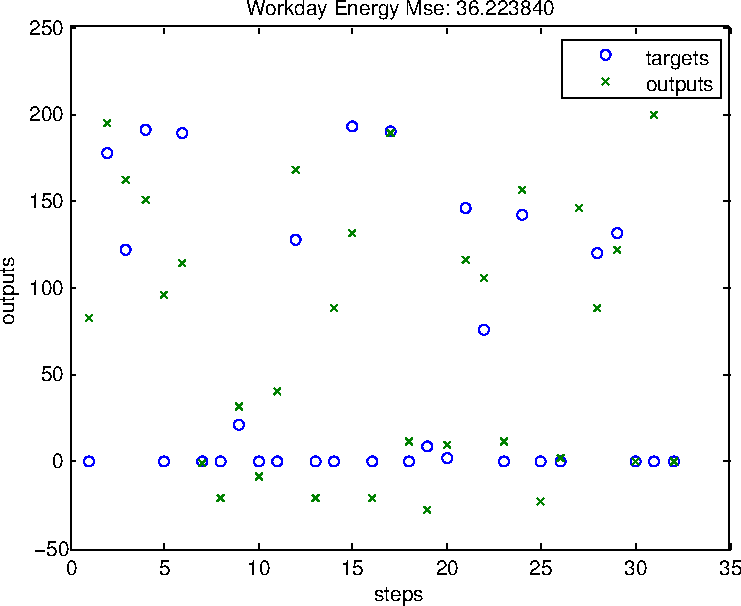
\includegraphics[scale=0.5]{images/anfis/workday/energy.pdf}
\captionof{figure}[One figure]{Energia consumata nei giorni feriali}
\vspace{20px}

La seguente tabella riporta invece i singoli errori (misurati come differenza tra target ed output) delle tre reti:

\begin{table}
  \caption{Risultati}
  \centering
	\begin{tabular}{lll}
		\toprule
    Giorni festivi (Energia) & Giorni feriali (Energia) & Giorni feriali (Luce interna) \\
		\midrule
    -3.4486 & -76.2742 & 31.3233 \\
    -52.2700 & -22.5364 & 16.1849 \\
    25.4036 & -28.7220 & 17.3464 \\
    -101.9807 & 0.9780 & 6.9155 \\
    -100.1104 & 6.3548 & -6.1994 \\
    6.2478 & -1.9842 & 0.7581 \\
    7.5718 & -8.8699 & 6.9155 \\
    -125.6459 & -78.3393 & -2.5798 \\
    -15.8978 & 20.8780 & -2.5798 \\
    -2.2610 & -7.6363 & -42.3179 \\
    -22.4493 & -6.3052 & 54.5844 \\
    -120.6839 & -54.9926 & 23.1033 \\
    2.4897 & 8.1659 & 6.0345 \\
    -1.1282 & -79.8701 & 44.4433 \\
    -4.1744 & -8.6983 & 87.5543 \\
    -9.0550 & -0.1074 & -36.0532 \\
    17.6492 & -44.0539 & 102.1473 \\
    7.8487 & -5.7140 & 3.0584 \\
    2.4897 & -36.5660 & -60.4570 \\
    64.2409 & -8.0969 & -1.3219 \\
    -1.1282 & -39.7330 & 9.3465 \\
    3.0565 & -5.7140 & 0.7581 \\
    0.6982 & -12.0171 & -2.5798 \\
    -4.2594 & 7.7194 & 6.9155 \\
    -46.1005 & -85.7398 & 13.8765 \\
    -35.9813 & -0.1074 & 3.0584 \\
    49.5614 & 29.6689 & -68.8789 \\
    1.3049 & -26.4973 & 4.9651 \\
    -3.2561 & 2.0773 & 64.5088 \\
    -14.3114 & -66.0939 & -15.0161 \\
    -1.1282 & 0.4544 & -6.1994 \\
    -1.1282 & -0.1074 & 0.7581 \\
		\bottomrule
	\end{tabular}
\end{table}

\clearpage


\section{Conclusioni}
\subsection{So una sega}

\subsection{Codice sorgente}


\end{document}
